
\part*{Bloque 1: Estimadores} \setcounter{chapter}{-1}
\chapter{Repaso}
\section{Variables aleatorias continuas}

\begin{definicion}[29]
Una función $f : \R \to \overline{\R}^+$ se llama \emph{de densidad} si $f(x) \ge 0$, es continua y
\[
  \int_{-\infty}^{\infty} f(x)\,dx = 1.
\]
\end{definicion}

\begin{proposicion}[55]
Supongamos que existe una función $f : \R \to \overline{\R}^+$ (de densidad) de modo que la función $F : \R \to \R^+$ viene dada por
\[
  F(x) = \int_{-\infty}^{x} f(x')\,dx'.
\]
Entonces:
\begin{enumerate}[label=(\alph*)]
  \item $F$ es una FdD asociada a una v.a.:
        \[
          0 = F(-\infty) \le F(x) \le F(\infty) = 1.
        \]
  \item $F(x)$ es de clase $C^1$ (función continua y diferenciable) con derivada $\partial_x F = f$.
  \item Para todo $x_0$:
        \[
          \Prob_X(\{x_0\}) \coloneqq \Prob(X = x_0) = \lim_{x \to x_0^+} F(x) - \lim_{x \to x_0^-} F(x) = 0.
        \]
\end{enumerate}
\end{proposicion}

\begin{proof}
El Th.\ de Barrow garantiza que $F(x)$ es de clase $C^1$, y con derivada $\partial_x F = f(x) \ge 0 \Rightarrow F\uparrow$. Luego $F\uparrow$ es creciente, $F(x)$ es de clase $C^1$ y por tanto $C^0$, por lo que no tiene discontinuidades.
\end{proof}

\begin{definicion}[30]
Una variable aleatoria $X : \Omega \to \R$ se llama \emph{continua} si:
\begin{enumerate}[label=(\alph*)]
  \item $\operatorname{Im} X = \aleph_1$, es decir, $\operatorname{Im} X = \R$ o $\operatorname{Im} X = (a,b)$, $a < b \in \R$.
  \item Existe una función $f : \R \to \overline{\R}^+$ (de densidad) de modo que $\Prob_X$ es la medida $\Prob_X : \mathcal{B} \to \R$ definida sobre la clase de los intervalos por
        \[
          \Prob_X(B) \coloneqq \Prob(X \in B) = \int_a^b f(x')\,dx', \qquad B = [a,b] \in \mathcal{B}.
        \]
\end{enumerate}
\end{definicion}

\begin{corolario}[3]
Si $X : \Omega \to \R$ es variable aleatoria continua se tiene también:
\begin{enumerate}[label=(\alph*)]
  \item Su FdD es
        \[
          F(x) = \Prob(X \le x) = \int_{-\infty}^{x} f(x')\,dx', \qquad
          \Prob(X \in [a,b]) = F(b) - F(a) = \int_{[a,b]} f(x')\,dx'.
        \]
  \item $\operatorname{Im} X = \aleph_1$ y contiene intervalos abiertos.
  \item Se define el soporte de la v.a.\ como $\operatorname{Sop} X = \{x \in \R : f(x) > 0\}$. Entonces $\operatorname{Im} X = \operatorname{Sop} X$ a.s.
\end{enumerate}
\end{corolario}

\begin{observacion}[34]
En contraste, existen variables aleatorias no continuas, las llamadas \emph{v.a.'s singulares}, tales que $S \coloneqq \operatorname{Im} X$ satisface:
\begin{enumerate}[label=(\alph*)]
  \item $\lambda(S) = 0$ (medida de Lebesgue nula).
  \item $\#S = \aleph_1$.
  \item $S$ no contiene intervalos abiertos.
  \item Es homeomorfo al conjunto de Cantor.
\end{enumerate}
\end{observacion}

\begin{observacion}[35]
A veces se afirma (o se interpreta) que $f(x) = \Prob(X = x)$. Esto es \textbf{falso} para v.a.c. De hecho, si $X$ es v.a.c.:
\begin{enumerate}[label=(\alph*)]
  \item $\Prob(X = x) = 0$, $\forall x$.
  \item $f(x)\,dx = \Prob(X \in [x, x+dx])$ o $f(x)\Delta x = \Prob(X \in [x, x+\Delta x])$.
  \item Existe un intervalo $I$ tal que $f(x) > 0$ si $x \in I$.
  \item $f(x) \ge 0$. Incluso puede ocurrir que $f(x) \ge 1$.
  \item Aunque no es normal, podría ocurrir que $f(x) = \infty$ en un conjunto numerable.
\end{enumerate}
\end{observacion}

\begin{definicion}[31]
Llamaremos \emph{soporte} de $X$ al conjunto $S_X \coloneqq \{x \in \R : f(x) > 0\}$.
\end{definicion}

\begin{proposicion}[56]
Si $X : \Omega \to \R$ es variable aleatoria continua, la esperanza o valor medio es
\[
  \E X \equiv \langle X \rangle \equiv \mu = \int_{\R} x\,f(x)\,dx.
\]
Además, si $g : \R \to \R$ es una función cualquiera y $Y = g \circ X$:
\[
  \E Y \equiv \E g(X) = \int_{\R} g(x)\,f(x)\,dx.
\]
\end{proposicion}

\begin{ejemplo}[30]
Supongamos que $a, b$ son constantes. Entonces
\[
  f(x) = \frac{1}{b-a}\,\chi_{[a,b]}(x)
\]
es una densidad: uniforme en el intervalo $[a,b]$. Además:
\[
  F(x) =
  \begin{cases}
    0, & x \le a, \\[4pt]
    \frac{x-a}{b-a}, & a \le x \le b, \\[4pt]
    1, & x \ge b.
  \end{cases}
\]
\end{ejemplo}

\begin{ejemplo}[31]
Supongamos que $\lambda > 0$ es constante. Entonces la densidad y distribución exponencial de parámetro $\lambda$ viene dada por
\[
  f(x) =
  \begin{cases}
    \lambda e^{-\lambda x}, & x \ge 0, \\
    0, & x \le 0,
  \end{cases}
  \qquad
  F(x) =
  \begin{cases}
    1 - e^{-\lambda x}, & x \ge 0, \\
    0, & x \le 0.
  \end{cases}
\]
\end{ejemplo}

\begin{figure}[htbp]
  \centering
  \begin{minipage}[b]{0.48\textwidth}
    \centering
    \begin{tikzpicture}[scale=0.85]
      \draw[->, thick] (0,0) -- (6,0) node[below] {$x$};
      \draw[->, thick] (0,0) -- (0,2.5) node[left] {$f(x)$};
      \node[below] at (0,0) {$0$};
      \node[below] at (2,0) {$a$};
      \node[below] at (4,0) {$b$};
      \draw[thick] (2,0) -- (2,1.2) -- (4,1.2) -- (4,0);
    \end{tikzpicture}
    \caption*{Figure 5: La función densidad de una variable uniforme}
  \end{minipage}
  \hfill
  \begin{minipage}[b]{0.48\textwidth}
    \centering
    \begin{tikzpicture}[scale=0.85]
      \draw[->, thick] (0,0) -- (6,0) node[below] {$x$};
      \draw[->, thick] (0,0) -- (0,2.5) node[left] {$F(x)$};
      \node[below] at (0,0) {$0$};
      \node[below] at (2,0) {$a$};
      \node[below] at (4,0) {$b$};
      \draw[thick] (2,0) -- (4,1.5) -- (6,1.5);
    \end{tikzpicture}
    \caption*{Figure 6: La función de distribución de una variable uniforme}
  \end{minipage}
\end{figure}

\begin{definicion}[32]
Supongamos que $\mu, \sigma$ son constantes. La \emph{densidad normal} de parámetros $\mu, \sigma$ se define por
\[
  f(x) = (2\pi\sigma^2)^{-\frac{1}{2}} e^{-(x-\mu)^2/(2\sigma^2)}.
\]
\end{definicion}

\begin{figure}[htbp]
  \centering
  \begin{minipage}[t]{0.48\textwidth}
    \centering
    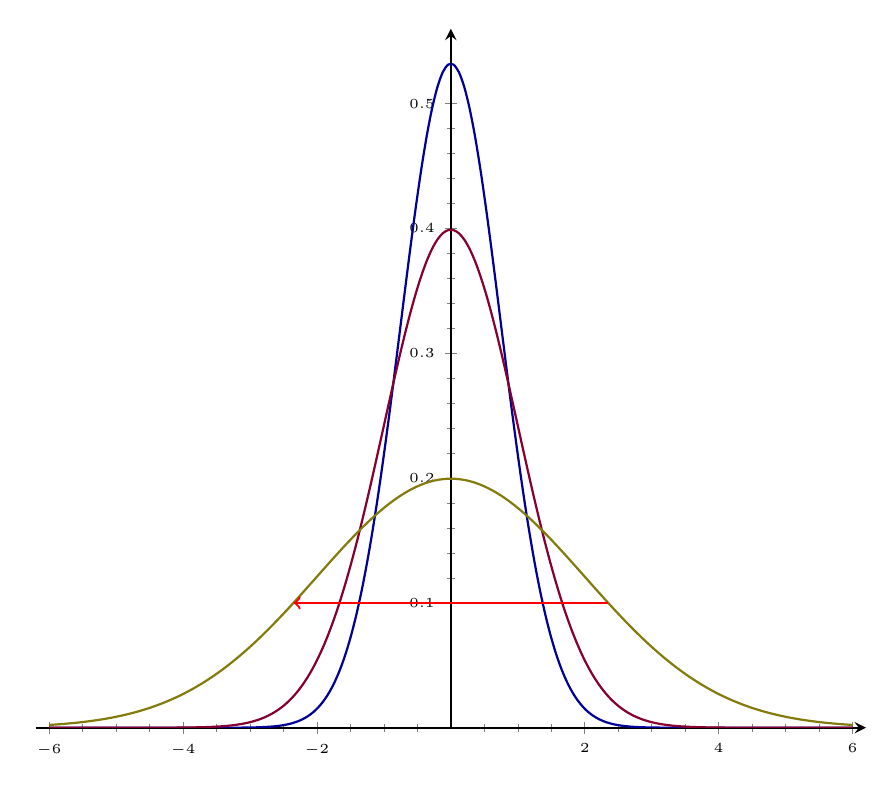
\begin{tikzpicture}
      \begin{axis}[
        width=\textwidth,
        axis lines=middle,
        xmin=-6.2, xmax=6.2,
        ymin=0, ymax=0.56,
        xtick={-6,-4,-2,0,2,4,6},
        ytick={0.1,0.2,0.3,0.4,0.5},
        minor x tick num=3,
        minor y tick num=4,
        tick label style={font=\tiny},
        domain=-6:6,
        samples=150,
        smooth,
        thick
      ]
        \addplot[color=blue!60!black] {1/(0.75*sqrt(2*pi))*exp(-x^2/(2*0.75^2))};
        \addplot[color=purple!70!black] {1/(1*sqrt(2*pi))*exp(-x^2/(2*1^2))};
        \addplot[color=olive!90!black] {1/(2*sqrt(2*pi))*exp(-x^2/(2*2^2))};
        \draw[->, red, thick] (axis cs:2.35, 0.1) -- (axis cs:-2.35, 0.1);
      \end{axis}
    \end{tikzpicture}
    \caption*{Figure 7: Campana de Gauss: densidad de probabilidad Gaussiana con $\mu=0$, $\sigma=0.75$, $\sigma=1$, $\sigma=2$}
  \end{minipage}
  \hfill
  \begin{minipage}[t]{0.48\textwidth}
    \centering
    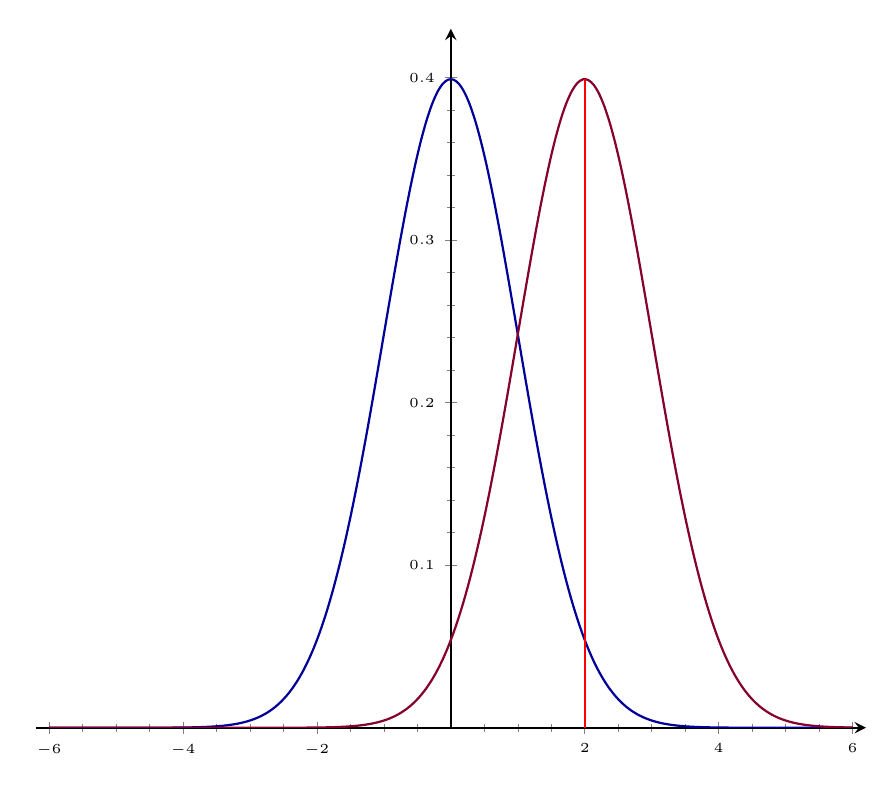
\begin{tikzpicture}
      \begin{axis}[
        width=\textwidth,
        axis lines=middle,
        xmin=-6.2, xmax=6.2,
        ymin=0, ymax=0.43,
        xtick={-6,-4,-2,0,2,4,6},
        ytick={0.1,0.2,0.3,0.4},
        minor x tick num=3,
        minor y tick num=4,
        tick label style={font=\tiny},
        domain=-6:6,
        samples=150,
        smooth,
        thick
      ]
        \addplot[color=blue!60!black] {1/sqrt(2*pi)*exp(-x^2/2)};
        \addplot[color=purple!70!black] {1/sqrt(2*pi)*exp(-(x-2)^2/2)};
        \draw[red, thick] (axis cs:2, 0) -- (axis cs:2, 0.3989);
      \end{axis}
    \end{tikzpicture}
    \caption*{Figure 8: Campana de Gauss: densidad de probabilidad Gaussiana con $\mu=0$, $\mu=2$}
  \end{minipage}
\end{figure}

\begin{proposicion}[57]
Supongamos que $X \sim \mathcal{N}(\mu, \sigma^2)$. Entonces:
\begin{enumerate}
  \item $f'(x) = 0 \Leftrightarrow x = \mu \coloneqq \arg\max f(x)$ \quad (máximo $=$ moda).
  \item $f''(x) = 0 \Leftrightarrow x = \mu \pm \sigma$ \quad (pto.\ de inflexión).
  \item $f(\mu + x) = f(\mu - x)$ \quad (simetría).
\end{enumerate}
\end{proposicion}

\begin{proposicion}[58]
Supongamos que $X \sim \mathcal{N}(\mu, \sigma^2)$. Entonces:
\begin{enumerate}
        \item   \textcolor{azulresalt}{\textbf{Tipificación:} $X \sim \mathcal{N}(\mu, \sigma^2) \Leftrightarrow Y \equiv \left(\frac{X-\mu}{\sigma}\right) \sim \mathcal{N}(0,1)$.
        Además sus funciones de distribución se relacionan por
        \[
          F_X(x) = F_Y\!\left(\frac{x-\mu}{\sigma}\right) \equiv \Phi\!\left(\frac{x-\mu}{\sigma}\right), \quad \forall x \in \R.
        \]}
  \item Cuando $X \sim \mathcal{N}(0,1)$ tenemos $\Pr(X \le x) = \Phi(x)$, donde $\Phi$ (la FdD de una v.a.\ $\mathcal{N}(0,1)$) es la función error dada por
        \[
          \Phi(x) = \int_{-\infty}^{x} (2\pi)^{-\frac{1}{2}} e^{-z^2/2}\,dz.
        \]
  \item Cuando $X \sim \mathcal{N}(\mu, \sigma^2)$ tenemos:
        \begin{align*}
          \Pr(X \le x) &= \int_{-\infty}^{x} f(z)\,dz = \Phi\!\left(\frac{x-\mu}{\sigma}\right), \\
          \Pr(X \in [a,b]) &= F(b) - F(a) = \Phi\!\left(\frac{b-\mu}{\sigma}\right) - \Phi\!\left(\frac{a-\mu}{\sigma}\right).
        \end{align*}
        Tomemos $a, b = \mu \pm n\sigma$, $n \in \N$. Entonces:
        \[
          \Pr(X \in [\mu - n\sigma, \mu + n\sigma]) = \Phi(n) - \Phi(-n) =
          \begin{cases}
            0{,}66, & n = 1, \\
            0{,}97, & n = 2, \\
            0{,}999, & n = 3.
          \end{cases}
        \]
  \item Más generalmente, si $Z = aX + b$, $a, b \in \R$, entonces $Z \sim \mathcal{N}(a\mu + b, \sigma^2 a^2)$.
\end{enumerate}
\end{proposicion}

\begin{figure}[htbp]
  \centering
  \begin{minipage}[t]{0.48\textwidth}
    \centering
    \begin{tikzpicture}
      \begin{axis}[
        width=\textwidth,
        axis lines=middle,
        xmin=-6.2, xmax=6.2,
        ymin=0, ymax=0.43,
        xtick={-6,-4,-2,0,2,4,6},
        ytick={0.1,0.2,0.3,0.4},
        minor x tick num=3,
        minor y tick num=4,
        tick label style={font=\tiny},
        samples=150,
        smooth
      ]
        \addplot[
          domain=-2:1,
          draw=red,
          thick,
          pattern=horizontal lines,
          pattern color=red
        ] {1/sqrt(2*pi)*exp(-x^2/2)} \closedcycle;
        \addplot[
          domain=-6:6,
          color=blue!60!black,
          thick
        ] {1/sqrt(2*pi)*exp(-x^2/2)};
      \end{axis}
    \end{tikzpicture}
    \caption*{Figure 9: $\Pr(x \in [-2, 1])$}
  \end{minipage}
  \hfill
  \begin{minipage}[t]{0.48\textwidth}
    \centering
    \begin{tikzpicture}
      \begin{axis}[
        width=\textwidth,
        axis lines=middle,
        xlabel={$x$},
        ylabel={$\operatorname{Erc}(x)$},
        xlabel style={right, font=\tiny},
        ylabel style={above, font=\tiny},
        xmin=-4.2, xmax=4.2,
        ymin=0, ymax=1.05,
        xtick={-4,-2,0,2,4},
        ytick={0.2,0.4,0.6,0.8,1.0},
        minor x tick num=3,
        minor y tick num=3,
        tick label style={font=\tiny},
        domain=-4:4,
        samples=150,
        smooth,
        thick
      ]
        \addplot[color=blue!60!black] {1/(1 + exp(-0.07056*x^3 - 1.5976*x))};
      \end{axis}
    \end{tikzpicture}
    \caption*{Figure 10: Función error o probabilidad acumulada bajo la curva densidad}
  \end{minipage}
\end{figure}

\begin{proof}
Supongamos $a > 0$ y sea $\psi(x) = ax + b \Rightarrow$ sabemos que $Z = \psi(X) \Rightarrow$
\begin{align*}
  F_Z(z) &= F_X(\psi^{-1}(z)) = F_X\!\left(\frac{z-b}{a}\right) \\
         &= (2\pi\sigma^2)^{-\nicefrac{1}{2}} \int_{-\infty}^{(z-b)/a} \exp\!\left(-\frac{(x-\mu)^2}{2\sigma^2}\right) dx \\
         &\overset{t=ax+b}{=} (2\pi\sigma^2 a^2)^{-\nicefrac{1}{2}} \int_{-\infty}^{z} \exp\!\left(-\frac{(t - \mu a - b)^2}{2\sigma^2 a^2}\right) dt \sim F_{\mathcal{N}(\mu a + b, \sigma^2 a^2)}(z).
\end{align*}
Esto prueba 4. Tomando $a = \frac{1}{\sigma}$ y $b = -\frac{\mu}{\sigma}$ se sigue el punto 1. Los demás son inmediatos.
\end{proof}

\begin{proposicion}[59]
Supongamos que $X \sim \mathcal{N}(0,1)$.
\begin{enumerate}
  \item $f(-x) = f(x)$; además $\Phi(-x) = 1 - \Phi(x)$.
  \item $\Prob(|X| \ge x) = \Prob(X \ge x) + \Prob(X \le -x) = 1 - \Phi(x) + \Phi(-x) = 2\Phi(-x) = 2(1 - \Phi(x))$.
  \item $\Prob(|X| \le x) = 2\Phi(x) - 1$. Si $p \in (0,1)$, los cuantiles cola son:
        \[
          \Prob(|X| \le x) = p \Leftrightarrow 2\Phi(x) - 1 = p \Leftrightarrow x = \Phi^{-1}\!\left(\frac{1+p}{2}\right).
        \]
  \item $Y = aX + b$, $a, b \in \R \Rightarrow Y \sim \mathcal{N}(b, a^2)$.
  \item $Y = X^2 \Rightarrow Y \sim \chi^2(1)$.
\end{enumerate}
\end{proposicion}

\begin{proof}[En efecto, para 5]
Tenemos $\operatorname{Sop} Y = [0, \infty)$. Dado $y > 0$:
\begin{align*}
  Y = X^2 \le y &\Rightarrow -\sqrt{y} \le X \le \sqrt{y} \Rightarrow F_Y(y) = \Prob(-\sqrt{y} \le X \le \sqrt{y}) = \Phi(\sqrt{y}) - \Phi(-\sqrt{y}) \\
                &= (2\pi)^{-\nicefrac{1}{2}} \int_{-\sqrt{y}}^{\sqrt{y}} \exp(-x^2/2)\,dx = 2(2\pi)^{-\nicefrac{1}{2}} \int_{0}^{\sqrt{y}} \exp(-x^2/2)\,dx.
\end{align*}
Derivando:
\[
  f_Y(y) = 2\frac{d}{dy}(2\pi)^{-\nicefrac{1}{2}} \int_{0}^{\sqrt{y}} \exp(-x^2/2)\,dx = 2(2\pi)^{-\nicefrac{1}{2}}(4y)^{-\nicefrac{1}{2}} e^{-y/2} = \frac{e^{-y/2}}{\sqrt{2\pi y}} \sim \chi^2(1).
\]
\end{proof}

\section{Momentos}
\[
  \E X^n = \E(\sigma Y + \mu)^n =
  \begin{cases}
    \mu, & n = 1, \\
    \sigma^2, & n = 2.
  \end{cases}
\]
De hecho:
\[
  \E X = \E(\sigma Y + \mu) = \mu + \sigma \E Y = \mu.
\]

\section{Cuantiles}

\begin{definicion}[60 — Cuantiles]
Dada una v.a.\ $X$ continua, la función de distribución es continua y estrictamente creciente en $\R$, tiene inversa bien definida y dado $p \in (0,1)$ los cuantiles se definen como
\[
  Q_p = \{x : F_X(x) = p\} = F_X^{-1}(p).
\]
En un caso general donde $F$ no tiene inversa bien definida, el conjunto $\{x : F_X(x) = p\}$ puede ser vacío o tener más de un punto. Definimos la función cuantil $Q : (0,1) \to \R$ como la inversa generalizada $Q \equiv F_X^{\leftarrow}$:
\[
  Q(p) \coloneqq Q_p = \inf\{x : \overline{F}_X(x) \coloneqq \Prob(X \ge x) \ge p\}.
\]
La función $\overline{F}(x) \coloneqq 1 - F(x)$ se denomina \emph{cola}. $\overline{F}(x)$ decrece desde $1$ a $0$. Los intervalos de constancia de $F$ se convierten en saltos de $Q \equiv F_X^{\leftarrow}$ y los saltos de $F$ en intervalos de constancia de $Q$.

La función cuantil de la distribución normal estándar se denomina \emph{función probit}, $\Phi^{-1}(p)$, $p \in (0,1)$, denotada como $z_p$.
\end{definicion}
\textcolor{azulresalt}{
\begin{proposicion}[60]
Si $p \in (0,1)$ y $z_p \coloneqq \Phi^{-1}(p)$:
\begin{enumerate}
  \item $\Prob(|X| \le x) = q \Leftrightarrow x = z_{(1+q)/2} \Leftrightarrow \Prob(|X| \le z_{(1+q)/2}) = q$.
  \item Si $q = 0{,}95$ entonces (ver figura):
        \[
          \Prob(X \ge x) = 0{,}025 \Leftrightarrow \Prob(X \le -x) = 0{,}025 \Leftrightarrow \Prob(|X| \ge x) = 0{,}05 \]
        \[ \Leftrightarrow \Prob(|X| \le x) = 0{,}95 \Leftrightarrow x = z_{0{,}975} = 1{,}96.
        \]
        Alternativamente, las observaciones se situarán fuera del intervalo $(-1{,}96, 1{,}96)$ en el $5\%$ de casos.
  \item $\Prob(|X| \ge x) = q \Leftrightarrow x = z_{1-q/2} \Leftrightarrow \Prob(|X| \ge z_{1-q/2}) = q \Leftrightarrow \Prob(|X| \ge z_q) = 2(1-q)$.
\end{enumerate}
\end{proposicion}}

\begin{proof}
$\Prob(|X| \le x) = 2\Phi(x) - 1 \Rightarrow \Prob(|X| \le x) = q \Leftrightarrow 2\Phi(x) - 1 = q \Leftrightarrow x = \Phi^{-1}((1+q)/2) \equiv z_{(1+q)/2}$.
\end{proof}

\begin{proposicion}[61]
Sea $X \sim \mathcal{N}(\mu, \sigma^2)$. Entonces:
\begin{enumerate}
  \item $F^{-1}(p) = \mu + \sigma \Phi^{-1}(p) \equiv \mu + \sigma z_p$, $p \in (0,1)$.
  \item $\Prob(X \ge \mu + \sigma z_p) = 1 - p$.
  \item $\Prob(X \notin (\mu - \sigma z_p, \mu + \sigma z_p)) = 2(1 - p)$.
  \item $X \sim \mathcal{N}(\mu, \sigma^2)$ se situará fuera del intervalo $(\mu - 1{,}96\sigma, \mu + 1{,}96\sigma)$ en el $5\%$ de casos.
\end{enumerate}
\end{proposicion}

\begin{figure}[htbp]
  \centering
  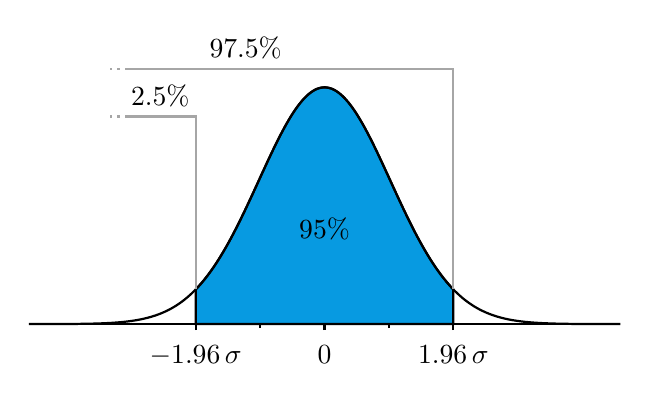
\begin{tikzpicture}
    \begin{axis}[
      width=0.75\textwidth,
      height=5.5cm,
      axis x line=bottom,
      axis y line=none,
      axis line style={-, thick},
      xmin=-4.5, xmax=4.5,
      ymin=0, ymax=0.52,
      xtick={-1.96, 0, 1.96},
      xticklabels={$-1.96\,\sigma$, $0$, $1.96\,\sigma$},
      minor x tick num=1,
      major tick style={black, thick},
      minor tick style={black, thick},
      xtick pos=bottom,
      tick label style={font=\normalsize, yshift=-2pt},
      samples=150,
      smooth,
      clip=false
    ]
      \addplot[
        domain=-1.96:1.96,
        fill=cyan!85!blue,
        draw=black,
        thick
      ] {1/sqrt(2*pi)*exp(-x^2/2)} \closedcycle;
      \addplot[
        domain=-4.5:4.5,
        color=black,
        thick
      ] {1/sqrt(2*pi)*exp(-x^2/2)};
      \node[font=\normalsize] at (axis cs:0, 0.16) {$95\%$};
      \draw[gray!70, thick] (axis cs:-1.96, 0.0584) -- (axis cs:-1.96, 0.35) -- (axis cs:-3.0, 0.35);
      \draw[gray!70, thick, dotted] (axis cs:-3.0, 0.35) -- (axis cs:-3.35, 0.35);
      \node[above, font=\normalsize] at (axis cs:-2.5, 0.35) {$2.5\%$};
      \draw[gray!70, thick] (axis cs:1.96, 0.0584) -- (axis cs:1.96, 0.43) -- (axis cs:-3.0, 0.43);
      \draw[gray!70, thick, dotted] (axis cs:-3.0, 0.43) -- (axis cs:-3.35, 0.43);
      \node[above, font=\normalsize] at (axis cs:-1.2, 0.43) {$97.5\%$};
    \end{axis}
  \end{tikzpicture}
  \caption*{Figura 1: Cuantiles para $q = 0.95$}
\end{figure}

\chapter{Leyes de grandes números y teorema central del límite}

En lo sucesivo consideramos un espacio de probabilidad $(\Omega, \mathcal{G}, \Prob)$ (ep) asociado a cierto experimento aleatorio (ea).

\begin{definicion}[13]
Un vector aleatorio $(X, Y)$ es una aplicación $\Omega \to \R^2$, $\omega \mapsto (X(\omega), Y(\omega))$, que a cada resultado $\omega$ del ea le asocia los valores $(X(\omega), Y(\omega)) \in \R^2$.
\end{definicion}

\begin{definicion}[14 — Distribución conjunta]
Sean $X, Y$ v.a. La función de distribución conjunta y las funciones de distribución marginales se definen por
\[
  F_{X,Y}(x,y) = \Prob(X \le x, Y \le y), \qquad F_X(x) \coloneqq \Prob(X \le x), \quad F_Y(y) \coloneqq \Prob(Y \le y), \quad \forall x,y \in \R.
\]
La función de distribución conjunta permite obtener las marginales mediante (ver Prop.\ 20):
\[
  F_X(x) = F_{X,Y}(x, \infty), \qquad F_Y(y) = F_{X,Y}(\infty, y).
\]
\end{definicion}

Hay tres tipos puros de vectores aleatorios en $\R^n$: discreto, continuo y singular.

\begin{definicion}[15]
Sean $X, Y$ v.a.\ discretas con soportes numerables $S_X \equiv \{x_n\}_{n=1}^\infty$, $S_Y \equiv \{y_n\}_{n=1}^\infty \subset \R$. Entonces el vector aleatorio $(X, Y)$ es también discreto. La función de masa conjunta es la distribución de probabilidad (en el plano)
\begin{equation*}
  \Prob_{X,Y}(x,y) \equiv \Prob(X = x, Y = y) \equiv f(x,y), \qquad x \in S_X, \; y \in S_Y.
\end{equation*}
El soporte de $X$ (o de la probabilidad $\Prob_X$) es el conjunto numerable $S_X = \{x \in \R : \Prob_X(x) > 0\}$.
El soporte del vector $(X, Y)$ (o de la probabilidad $\Prob_{X,Y}$) es el conjunto numerable
\[
  S = \{(x,y) \in \R^2 : \Prob_{X,Y}(x,y) > 0\} \equiv \{(x_n, y_m)\} \subset S_X \times S_Y \subset \R^2.
\]
Es conveniente escribir $\Prob(X = x, Y = y) \equiv f(x,y)$, pero $f$ no es una densidad bivariante.
\end{definicion}

\begin{definicion}[16]
El vector aleatorio $(X, Y)$ es de tipo continuo —o tiene densidad conjunta bivariante— si existe $f : \R^2 \to \R^+$, $(x,y) \mapsto f(x,y)$ continua (salvo un conjunto finito de puntos) de modo que
\[
  f(x,y) \ge 0, \quad f \in C^0, \quad \iint_{\R^2} f(x,y)\,dx\,dy = 1
\]
y $\forall B \subset \R^2$ es
\begin{equation*}
  \Prob((X, Y) \in B) = \iint_B f(x,y)\,dx\,dy.
\end{equation*}
En este caso:
\begin{equation*}
  F(x,y) \coloneqq \Prob(X \le x, Y \le y) = \int_{-\infty}^x \int_{-\infty}^y f(x', y')\,dx'\,dy'; \qquad f(x,y) = \frac{\partial^2 F}{\partial x \partial y}(x,y).
\end{equation*}
El soporte de la probabilidad conjunta es la región bidimensional
\[
  S = \{(x,y) : f(x,y) > 0\} \subset \R^2.
\]
\end{definicion}
\textcolor{azulresalt}{
\begin{proposicion}[19]
Sea $R$ un rectángulo de vértices $v_i = (a_1, b_1), (a_2, b_1), (a_1, b_2), (a_2, b_2)$. La función de distribución conjunta satisface
\[
  \Prob((X, Y) \in R) = \Prob(a_1 \le X \le a_2, b_1 \le Y \le b_2) = F(a_2, b_2) - F(a_1, b_2) - F(a_2, b_1) + F(a_1, b_1).
\]
En particular, si $F(x,y)$ es independiente de $y$ (o $x$) en una región $D$, entonces para todo rectángulo $R \subset D$ es $\Prob((X, Y) \in R) = 0$.
\end{proposicion}
\begin{proof}
Usar representación integral.
\end{proof}}

\begin{proposicion}[20]
Si existe la densidad conjunta $f(x,y)$, entonces $X, Y$ tienen densidades marginales $f_X(x)$, $f_Y(y)$:
\begin{equation*}
  f_X(x) = \int_{-\infty}^\infty f(x,y)\,dy, \qquad f_Y(y) = \int_{-\infty}^\infty f(x,y)\,dx.
\end{equation*}
Sin embargo, que $X, Y$ tengan densidades marginales $f_X(x)$, $f_Y(y)$ no implica necesariamente que exista la densidad conjunta $f(x,y)$.
\end{proposicion}

\begin{proof}
\[
  F_X(x) \coloneqq \Prob(X \le x) = \Prob(X \le x, Y \in \R) = \int_{-\infty}^x \int_{-\infty}^\infty f(x', y)\,dx'\,dy = \int_{-\infty}^x f_X(x')\,dx'
\]
donde $f_X(x') \equiv \int_{-\infty}^\infty f(x', y)\,dy$ es una densidad unidimensional (probar). Se sigue que
\begin{equation*}
  f_X(x) = \int_{-\infty}^\infty f(x,y)\,dy, \qquad F_X(x) = F_{X,Y}(x, \infty).
\end{equation*}
\end{proof}

\begin{ejemplo}[20]
Distribución bidimensional normal estándar de parámetro $\rho \in (-1, 1)$ y soporte $\R^2$:
\[
  \mathcal{N}(0, 1, 0, 1; \rho) \implies f(x,y) = \left(2\pi\sqrt{1-\rho^2}\right)^{-1} e^{-(x^2 - 2xy\rho + y^2)/(2(1-\rho^2))}.
\]
\end{ejemplo}

\begin{definicion}[17]
Si $X : \Omega \to \R$ es variable aleatoria continua, la esperanza o valor medio es
\[
  \E X \equiv \langle X \rangle \equiv \mu = \int_{\R} x\,f(x)\,dx.
\]
Además, si $T : \R \to \R$ es una función cualquiera y $Y = T \circ X$:
\[
  \E Y \equiv \E T(X) = \int_{\R} T(x)\,f(x)\,dx.
\]
Finalmente, si $T : \R^2 \to \R$ es una función cualquiera y existe la densidad conjunta $f(x,y)$:
\begin{equation*}
  \E(T(X,Y)) = \iint_{\R^2} T(x,y)\,f(x,y)\,dx\,dy.
\end{equation*}
El caso discreto se obtiene cambiando integrales por sumas e interpretando $f(x,y)$ como la función de masa:
\begin{equation*}
  \E(T(X,Y)) = \sum_n \sum_m T(x_n, y_m)\,f(x_n, y_m).
\end{equation*}
\end{definicion}

\begin{definicion}[18]
Dos variables aleatorias $X, Y$ son independientes: $X \indep Y \iff$ se cumple alguna de las condiciones:
\begin{enumerate}
  \item El conocimiento de una no proporciona \emph{ninguna información} sobre la otra, o
  \item Si lo son los sucesos $B_1 = \{X \le x\}$, $B_2 = \{Y \le y\}$, $\forall x,y$, es decir, si
        \begin{equation*}
          F_{X,Y}(x,y) \equiv \Prob(X \le x, Y \le y) = \Prob(X \le x)\Prob(Y \le y) \equiv F_X(x)F_Y(y), \quad \forall x,y \in \R.
        \end{equation*}
  \item $\iff f_{X,Y}(x,y) = f_X(x) \cdot f_Y(y)$, $\forall x,y \in \R$, donde $f_X(x)$ es la función de masa o bien de densidad (caso continuo).
  \item Para toda función $g_1, g_2 : \R \to \R$ es $g_1(X) \indep g_2(Y)$, y
        \[
          \iff \E(g_1(X) \cdot g_2(Y)) = \E(g_1(X)) \cdot \E(g_2(Y)).
        \]
\end{enumerate}
\end{definicion}

\begin{definicion}[19]
Dos variables aleatorias $X, Y$ están idénticamente distribuidas: $X \stackrel{D}{=} Y$ sii
\[
  F_X(x) = F_Y(x), \quad \forall x \in \R.
\]
La relación $X \stackrel{D}{=} Y \iff F_X(x) = F_Y(x)$ $\forall x \in \R$ es de equivalencia. Diremos que las variables aleatorias $X, Y, \dots$ son i.i.d.\ si están idénticamente distribuidas y son independientes.
\end{definicion}

\begin{ejemplo}
Sean $X, Y$ el número de caras (cruces) en $n$ tiradas de una moneda justa. Entonces $X, Y \sim \operatorname{Bin}(n, \frac{1}{2})$ están idénticamente distribuidas, pero si $n$ es impar es siempre $X \neq Y$. Es decir, la relación de equivalencia $X \sim Y \iff F_X(x) = F_Y(x)$ $\forall x \in \R$ no implica $X = Y$. Tampoco es $X \indep Y$ pues $Y = n - X$.
\end{ejemplo}

\begin{teorema}[1 — Desigualdad de Markov]
Sea $X$ una v.a. Entonces $\forall M$, $\forall \varphi$ con $\varphi : \R \to \R^+$, $\varphi(x) > 0$ $\forall x \neq 0$, $\varphi(x)\uparrow$, se verifica que
\[
  \Prob(|X| \ge M) \le \frac{\E(\varphi(|X|))}{\varphi(M)}.
\]
En particular:
\begin{enumerate}
  \item \textbf{Markov:} $\Prob(|X| \ge M) \le \dfrac{\E|X|^n}{M^n}$, $\forall n$.
  \item \textbf{Chebyshev:} $\Prob(|X - \mu_X| \ge M) \le \dfrac{\Var(X)}{M^2}$.
\end{enumerate}
\end{teorema}
\textcolor{red}{
\begin{proof}
$\varphi(x)\uparrow$, luego si $a \equiv \varphi(M)$ y $\vartheta(X) \coloneqq \varphi(|X|)/a$:
\begin{enumerate}
  \item $|X| \ge M \iff \varphi(|X|) \ge \varphi(M) \iff \vartheta(X) \ge 1$.
  \item $\vartheta(X) \ge 1$ en $\{\varphi(|X|)/a \ge 1\}$, i.e.\ en $\{\varphi(|X|) \ge a\}$.
  \item $\Prob(A) = \E \mathbf{1}_A$:
        \begin{align*}
          \Prob(|X| \ge M) &= \Prob(\varphi(|X|) \ge \varphi(M)) = \E\mathbf{1}_{\{\varphi(|X|) \ge \varphi(M)\}} = \E\mathbf{1}_{\{\vartheta(X) \ge 1\}} \\
                           &\le \E(\vartheta(X)\mathbf{1}_{\{\vartheta(X) \ge 1\}}) \le \frac{1}{a}\E(\varphi(|X|)\mathbf{1}_{\{\vartheta(X) \ge 1\}}) \le \frac{1}{a}\E(\varphi(|X|)).
        \end{align*}
\end{enumerate}
\end{proof}}

\begin{definicion}[26]
Sea $X$ una v.a. Se llama \emph{función característica} (fc) de la v.a.\ $X$ a la función
\begin{equation*}
  \phi_X(s) : \R \to \C, \qquad \phi_X(s) \coloneqq \E(e^{isX}), \quad s \in \R.
\end{equation*}
Si $X$ es una v.a.\ continua, la función característica es la transformada de Fourier de la densidad $f_X(x)$:
\begin{equation*}
  \E(e^{isX}) = \int_{-\infty}^\infty e^{isx} f_X(x)\,dx, \quad s \in \R.
\end{equation*}
Si $X$ es una v.a.\ discreta soportada en los naturales, la función característica es la ``transformada-$z$'' de la función de masa $(p_n)$ o función generatriz de la función de masa:
\begin{equation*}
  \E(e^{isX}) = \sum_{n=1}^\infty p_n z^n, \quad \text{donde } s \in \R^+, \; z \equiv e^{is}, \; |z| = 1.
\end{equation*}
\end{definicion}

\begin{teorema}[7 — Inversión de la transformada de Fourier]
Sea $X$ una v.a.\ continua con densidad $f_X(x)$. Supongamos que la función característica está en $L_1$, $\int_{-\infty}^\infty |\phi(s)|\,ds < \infty$; entonces:
\[
  f_X(x) = \frac{1}{2\pi} \int_{-\infty}^\infty e^{-isx} \phi(s)\,ds.
\]
\end{teorema}

\begin{teorema}[8]
Si $f$ decae lo suficientemente rápido para que los momentos existan, se tiene
\[
  \phi(0) = 1; \quad \phi'(0) = i\mu; \quad \dots \quad \phi^{(n)}(0) = i^n \mu_n \equiv i^n \int_{-\infty}^\infty x^n f_X(x)\,dx,
\]
y por tanto $\phi(s)$ tiene el desarrollo de Taylor en el origen:
\[
  \phi(s) = 1 + i\mu s - \frac{\sigma^2 s^2}{2} + \dots + \frac{i^n \mu_n s^n}{n!} + \dots
\]
\end{teorema}

\begin{proof}[Demostración]
Desarrollo en serie: es derivar formalmente $\left(\frac{d}{ds} e^{isx} = ix e^{isx}\right)$:
\begin{equation*}
  \phi'(0) = \left.\left(\frac{d}{ds} \int_{-\infty}^\infty e^{isx} f_X(x)\,dx\right)\right|_{s=0} = \left.\left(\int_{-\infty}^\infty ix e^{isx} f_X(x)\,dx\right)\right|_{s=0} = i\int_{-\infty}^\infty x f_X(x)\,dx = i\mu.
\end{equation*}
\end{proof}

\noindent \textbf{Ejemplos:}
\begin{enumerate}
  \item La función característica de una variable exponencial $\operatorname{Exp}(\lambda)$ es
        \[
          \phi(s) = \int_0^\infty \lambda e^{-\lambda x} e^{isx}\,dx = \left(1 - \frac{is}{\lambda}\right)^{-1},
        \]
        que tiene un polo en $s = -i\lambda$; la inversión se hace por el Th.\ de los residuos, que muestra que
        \[
          f_X(x) = \frac{1}{2\pi}\int_{-\infty}^\infty \frac{e^{-isx}}{1 - is/\lambda}\,ds =
          \begin{cases}
            \lambda e^{-\lambda x}, & x \ge 0, \\
            0, & x < 0.
          \end{cases}
        \]
  \item La función característica de una variable $\mathcal{N}(\mu, \sigma^2)$ es
        \[
          \phi(s) = \frac{1}{\sqrt{2\pi\sigma^2}}\int_{-\infty}^\infty e^{-(x-\mu)^2/(2\sigma^2) + isx}\,dx = e^{i\mu s - \sigma^2 s^2/2}.
        \]
        El cálculo se hace por técnicas de variable compleja.
  \item La función característica de una variable degenerada $\mathcal{D}(x_0)$ es $\E(e^{isX}) = e^{ix_0 s}$, que se puede obtener como límite de una normal con media $x_0$ y varianza $\sigma^2 \to 0$:
        \[
          e^{ix_0 s - \sigma^2 s^2/2} \xrightarrow{\sigma^2 \to 0} e^{ix_0 s}.
        \]
        Supongamos que $(X_n)_{n=1}^\infty \sim \mathcal{N}(\mu, \sigma^2/n)$; la función característica satisface
        \[
          \phi_{X_n}(s) = e^{i\mu s - \sigma^2 s^2/(2n)} \xrightarrow{n \to \infty} e^{i\mu s} \sim \mathcal{D}(\mu).
        \]
        Por el teorema de Lévy ($\phi_{X_n}(s) \xrightarrow{n \to \infty} \phi_{X_\infty}(s) \iff F_{X_n}(x) \xrightarrow{n \to \infty} F_{X_\infty}(x)$) se sigue que
        \[
          \lim_{n \to \infty} F_{X_n}(x) = F_{\mathcal{D}(\mu)}(x) =
          \begin{cases}
            1, & x \ge \mu, \\
            0, & x < \mu.
          \end{cases}
        \]
  \item Sea $X \sim \mathcal{N}(0,1)$ y sea $Y = X^2 \sim \chi^2(1)$. Su función característica es
        \[
          \phi(s) = \frac{1}{\sqrt{1 - 2is}}.
        \]
\end{enumerate}

\section{El problema de la suma}

En estadística la propiedad $X_i \sim \mathcal{N}(\mu_i, \sigma_i^2)$, $i=1,2 \Rightarrow X_1 + X_2 \sim \mathcal{N}(\mu_1 + \mu_2, \sigma_1^2 + \sigma_2^2)$ se usa a diario. ¿Es siempre verdad? ¿De dónde ha salido esto?

Dadas dos v.a.s $X_i$ con densidades $f_{X_i}(x)$, un problema natural de la estadística es calcular la densidad de la suma $f_{X_1 + X_2}(x)$. Este es un problema no trivial pero que se simplifica mucho si: (i) las $X_i$ son v.a.s independientes; (ii) pertenecen a una familia reproductiva.

\begin{teorema}[9]
Sean $(X_1, \dots, X_n, \dots)$ v.a.s independientes. Entonces la función característica de la suma $Y \coloneqq X_1 + \dots + X_n$ es el producto de funciones características:
\[
  \phi_Y(s) = \phi_{X_1}(s) \cdots \phi_{X_n}(s).
\]
Si $(X_1, \dots, X_n, \dots)$ son i.i.d.:
\[
  \phi_Y(s) = (\phi_{X_1}(s))^n.
\]
\end{teorema}

\begin{proof}
Tenemos $e^{isY} = e^{isX_1 + \dots + isX_n} = e^{iX_1 s} \cdots e^{iX_n s}$. Además por independencia es un producto de independientes: $e^{iX_1 s} \indep \dots \indep e^{iX_n s}$. Luego
\[
  \E e^{isY} = \E(e^{iX_1 s} \cdots e^{iX_n s}) = \E e^{iX_1 s} \cdots \E e^{iX_n s} = \phi_{X_1}(s) \cdots \phi_{X_n}(s).
\]
\end{proof}
\textcolor{azulresalt}{
\begin{definicion}[27 — Reproductividad]
Diremos que una familia de v.a.s $(X_\theta)$ que depende de un parámetro $\theta$ con función característica $\phi(s; \theta)$ es \emph{reproductiva} si existe $g : \R^2 \to \R$ de modo que (ley de grupoide)
\[
  \phi(s; \theta_1) \cdot \phi(s; \theta_2) = \phi(s; \theta') \quad \text{donde } \theta' = g(\theta_1, \theta_2).
\]
Alternativamente, sea una familia de v.a.s $(X_\theta)$ cuya distribución de probabilidad $\Prob_{X_i; \theta}$ depende de un parámetro $\theta$. Diremos que $\Prob_{X_i; \theta}$ es reproductiva si dadas dos tales v.a.s independientes su suma tiene distribución $\Prob_{X_1; \theta'}$ donde $\theta' = g(\theta_1, \theta_2)$: $\Prob_{X_1 + X_2; \theta} = \Prob_{X_1; \theta'}$.
\end{definicion}}

\textcolor{azulresalt}{
\begin{ejemplo}[9]
Sean $X_i \sim \mathcal{N}(\mu_i, \sigma_i^2)$, $i=1,2$ independientes. Entonces es reproductiva pues $X_1 + X_2 \sim \mathcal{N}(\mu_1 + \mu_2, \sigma_1^2 + \sigma_2^2)$ con $\theta = (\mu, \sigma^2)$; $g(\theta_1, \theta_2) = \theta_1 + \theta_2$.
\end{ejemplo}}

\textcolor{azulresalt}{
\begin{proposicion}[18 — Suma y Reproductividad]
Dadas $X_i \sim \mathcal{N}(\mu_i, \sigma_i^2)$, $i=1,\dots,n$ independientes:
\begin{enumerate}
  \item $X_1 + \dots + X_n \sim \mathcal{N}\!\left(\sum_i \mu_i, \sum_i \sigma_i^2\right)$.
  \item Si $\mu_i = 0$ y $\sigma_i^2 = 1$, entonces $X_1^2 + \dots + X_n^2 \sim \chi^2(n)$.
\end{enumerate}
\end{proposicion}
}
\subsection{Distribuciones estadísticas notables}

\textcolor{azulresalt}{
\begin{definicion}[28]
La distribución exponencial $\operatorname{Exp}(\lambda)$ tiene densidad
\[
  f_X(x) =
  \begin{cases}
    \lambda e^{-\lambda x}, & x \ge 0, \\
    0, & x < 0.
  \end{cases}
\]
\end{definicion}
}

\textcolor{azulresalt}{
\begin{definicion}[29]
La distribución Gamma $\Gamma(\alpha, \beta)$ tiene densidad
\[
  f_{\Gamma(\alpha,\beta)}(x; \alpha, \beta) = \frac{x^{\alpha-1} e^{-\beta x} \beta^\alpha}{\Gamma(\alpha)} \quad \text{para } x > 0, \; \alpha, \beta > 0,
\]
donde $\Gamma(\cdot)$ denota la función Gamma.
\end{definicion}
}

\textcolor{azulresalt}{
\begin{definicion}[30]
La distribución $\chi^2(k)$ chi-cuadrado con $k$ grados de libertad tiene densidad
\[
  f_{\chi^2(k)}(x; k) =
  \begin{cases}
    \dfrac{x^{\nicefrac{k}{2} - 1} e^{-x/2}}{2^{\nicefrac{k}{2}}\Gamma\left(\frac{k}{2}\right)}, & x > 0, \\[6pt]
    0, & x < 0.
  \end{cases}
\]
\end{definicion}}

\textcolor{azulresalt}{
\begin{definicion}[31]
La distribución Erlang $\operatorname{Er}(k, \beta)$ tiene densidad
\[
  f_{\operatorname{Er}(k,\beta)}(x; k, \beta) = \frac{\beta^k x^{k-1} e^{-\beta x}}{(k-1)!}, \quad x > 0, \; \beta \ge 0, \; k \in \N.
\]
\end{definicion}}

\textcolor{azulresalt}{
Notar que $f_{\chi^2(k)} = f_{\Gamma(\nicefrac{k}{2}, \nicefrac{1}{2})}$, mientras que $f_{\operatorname{Er}(k,\beta)}$ se obtiene cuando $\alpha = k$ es un entero. Además $f_{\operatorname{Er}(1,\beta)}(x; 1, \beta) = \beta e^{-\beta x}$, $\beta \ge 0$, distribución exponencial.}

\section{Convergencia}

\begin{definicion}[32]
La sucesión $X_1, \dots, X_n, \dots$ converge c.s.\ hacia $X_\infty$:
\[
  X_n \xrightarrow[n\to\infty]{\text{c.s.}} X_\infty \iff X_n(\omega) \xrightarrow{n\to\infty} X_\infty(\omega), \quad \forall \omega \text{ salvo en un conjunto nulo } \omega \in N \mid \Prob(N) = 0.
\]
\end{definicion}

\begin{definicion}[33]
La sucesión $(X_n)_{n=1}^\infty$ converge hacia $X_\infty$ en probabilidad:
\[
  X_n \xrightarrow[n\to\infty]{\Prob} X_\infty \iff \lim_{n\to\infty} \Prob(|X_n - X_\infty| \ge \epsilon) = 0, \quad \forall \epsilon > 0.
\]
\end{definicion}

\begin{definicion}[28]
La sucesión $(X_n)_{n=1}^\infty$ converge hacia $X_\infty$ en sentido $L_r$, $r > 0$, si
\[
  X_n \xrightarrow[n\to\infty]{L_r} X_\infty \iff \lim_{n\to\infty} \E(|X_n - X_\infty|^r) = 0.
\]
En particular, la sucesión $(X_n)_{n=1}^\infty$ converge hacia $X_\infty$ en media cuadrática si lo hace en sentido $L_2$:
\[
  X_n \xrightarrow[n\to\infty]{L_2} X_\infty \iff \lim_{n\to\infty} \E(|X_n - X_\infty|^2) = 0.
\]
$(X_n)_{n=1}^\infty$ converge hacia $X_\infty$ en sentido $L_1$:
\[
  X_n \xrightarrow[n\to\infty]{L_1} X_\infty \iff \lim_{n\to\infty} \E(|X_n - X_\infty|) = 0.
\]
\end{definicion}

\begin{definicion}[29]
La sucesión $(X_n)_{n=1}^\infty$ converge hacia $X_\infty$ en distribución (tb llamada débil $D$) si
\[
  X_n \xrightarrow[n\to\infty]{D} X_\infty \iff \lim_{n\to\infty} F_{X_n} = F_{X_\infty}.
\]
\end{definicion}
\textcolor{azulresalt}{
Otras definiciones son:
\begin{definicion}[30]
$(X_n)_{n=1}^\infty$ converge c.s.\ hacia $X_\infty$ en sentido completo si
\[
  X_n \xrightarrow[n\to\infty]{\text{completo}} X_\infty \iff \sum_{n=1}^\infty \Prob(|X_n - X_\infty| \ge \epsilon) < \infty, \quad \forall \epsilon > 0.
\]
Su interés radica en que es una condición sencilla de comprobar y si se cumple implica convergencia c.s.
\end{definicion}}

\textcolor{azulresalt}{
\begin{definicion}[31]
$(X_n)_{n=1}^\infty$ converge hacia $X_\infty$ en media si lo hacen sus esperanzas:
\[
  \lim_{n\to\infty} \E X_n = \E X_\infty.
\]
Es un modo de convergencia natural y sencillo de comprobar.
\end{definicion}}

La convergencia c.s.\ es el modo más importante, pero técnicamente muy sofisticado. Los demás modos son auxiliares y modos de convergencia débiles.

\begin{teorema}[5 — Continuidad de Lévy]
La sucesión $(X_n)_{n=1}^\infty$ converge hacia $X_\infty$ en distribución si y solo si la sucesión $\phi_{X_n}$ converge a una función $\phi$ continua en el origen, que será entonces la fc de $X_\infty$:
\[
  X_n \xrightarrow[n\to\infty]{D} X_\infty \iff \lim_{n\to\infty} \phi_{X_n}(s) = \phi_{X_\infty}(s).
\]
\end{teorema}

\begin{teorema}[6]
Supongamos que $(X_n)_{n=1}^\infty$ converge en sentido completo hacia $X_\infty$. Entonces converge c.s.\ hacia $X_\infty$.
\end{teorema}

\begin{teorema}[7]
Supongamos que $(X_n)_{n=1}^\infty$ converge c.s.\ hacia $X_\infty$. Entonces $X_1, \dots, X_n, \dots$ converge hacia $X_\infty$ en probabilidad.
\end{teorema}

\begin{teorema}[8]
Supongamos que $(X_n)_{n=1}^\infty$ converge hacia $X_\infty$ en probabilidad. Entonces converge hacia $X_\infty$ en distribución:
\[
  \lim_{n\to\infty} |F_{X_n}(x) - F_{X_\infty}(x)| = 0, \quad \forall x.
\]
\end{teorema}

\begin{teorema}[9]
Supongamos que $(X_n)_{n=1}^\infty$ converge en sentido $L_1$ hacia $X_\infty$. Entonces converge hacia $X_\infty$ en media, aunque el recíproco no es cierto.
\end{teorema}

\begin{teorema}[10]
Supongamos que $(X_n)_{n=1}^\infty$ converge hacia $X_\infty$ en media cuadrática (es decir, en $L_2$). Entonces converge hacia $X_\infty$ en probabilidad.
\end{teorema}

\begin{proof}
Usando la desigualdad de Markov, dado $\epsilon > 0$:
\[
  \lim_{n\to\infty} \Prob(|X_n - X_\infty| \ge \epsilon) \le \lim_{n\to\infty} \frac{\E(X_n - X_\infty)^2}{\epsilon^2} = 0.
\]
El recíproco es falso: que $(X_n)_{n=1}^\infty$ converja hacia $X_\infty$ en distribución sólo dice que $\lim_{n\to\infty} X_n$ y $X_\infty$ tienen idéntica distribución, pero nada más. (Ver ejemplos).
\end{proof}

\begin{observacion}[8]
Convergencia casi segura no implica convergencia $L_1$ ni tampoco de las medias. Ver contraejemplo.
\end{observacion}

\begin{proposicion}[22]
Supongamos que $(X_n)_{n=1}^\infty$:
\begin{enumerate}
  \item converge hacia una constante $\theta$ en media: $\lim_{n\to\infty} \E X_n = \theta$,
  \item las varianzas convergen a $0$: $\lim_{n\to\infty} \Var X_n = \lim_{n\to\infty} \E(X_n - \E X_n)^2 = 0$.
\end{enumerate}
Entonces $(X_n)_{n=1}^\infty$ converge hacia $\theta$ en media cuadrática y en probabilidad. (Resultado muy usado en EM para establecer consistencia).
\end{proposicion}

\begin{proof}
Sea $\mu_n \coloneqq \E X_n$:
\begin{align*}
  \Var X_n &= \E(X_n - \theta + \theta - \mu_n)^2 = \E(X_n - \theta)^2 + \E(\theta - \mu_n)^2 + 2\E(X_n - \theta)\E(\theta - \mu_n) \\
           &\Rightarrow \E(X_n - \theta)^2 = \Var X_n + (\theta - \mu_n)^2 \\
           &\Rightarrow \lim_{n\to\infty} \E(X_n - \theta)^2 = \lim_{n\to\infty} \Var X_n + \lim_{n\to\infty} (\theta - \mu_n)^2 = 0 + 0 = 0.
\end{align*}
Además, por la desigualdad de Markov:
\[
  \lim_{n\to\infty} \Prob(|X_n - \theta| \ge \epsilon) \le \lim_{n\to\infty} \frac{\E(X_n - \theta)^2}{\epsilon^2} = 0.
\]
\end{proof}

\begin{teorema}[11]
Se verifican las siguientes relaciones de convergencia para $X_n \xrightarrow{n\to\infty} X_\infty$:
\begin{enumerate}
  \item $X_n \xrightarrow[n\to\infty]{\text{completo}} X_\infty \Rightarrow X_n \xrightarrow[n\to\infty]{\text{c.s.}} X_\infty$.
  \item $X_n \xrightarrow[n\to\infty]{\text{c.s.}} X_\infty \Rightarrow X_n \xrightarrow[n\to\infty]{\Prob} X_\infty \Rightarrow X_n \xrightarrow[n\to\infty]{D} X_\infty$.
  \item $X_n \xrightarrow[n\to\infty]{L_r} X_\infty \Rightarrow X_n \xrightarrow[n\to\infty]{\Prob} X_\infty$ ($r \ge 1$).
  \item $X_n \xrightarrow[n\to\infty]{D} X_\infty \iff X_n \xrightarrow[n\to\infty]{\text{fc}} X_\infty$.
  \item Si $X_\infty$ es constante y $X_n \xrightarrow[n\to\infty]{D} X_\infty \Rightarrow X_n \xrightarrow[n\to\infty]{\Prob} X_\infty$.
\end{enumerate}
\end{teorema}

\begin{teorema}[12 — \underline{Ley débil de grandes números}]
Sean $(X_n)_{n=1}^\infty$ sucesión i.i.d.\ con media $\mu \coloneqq \E X_1 \in (-\infty, \infty)$ y varianza finita $\Var X_1 = \sigma^2 < \infty$. Sea
\[
  M_n \equiv \overline{X}_n \coloneqq \frac{X_1 + \dots + X_n}{n} \quad (\text{media muestral}).
\]
Entonces se verifica que:
\[
  M_n \xrightarrow[n\to\infty]{D} \mu; \qquad M_n \xrightarrow[n\to\infty]{\Prob} \mu; \qquad M_n \xrightarrow[n\to\infty]{L_2} \mu.
\]
En estadística $M_n$ se denomina media muestral. Por tanto, la media muestral (el promedio estadístico) converge a la esperanza matemática.
\end{teorema}

\begin{proof}
\textbf{Convergencia en distribución:} Por independencia y equidistribución tendremos:
\begin{enumerate}
  \item $e^{isM_n} = e^{iX_1 s/n} \cdots e^{iX_n s/n}$.
  \item $e^{iX_1 s/n} \indep \dots \indep e^{iX_n s/n}$.
  \item $\E e^{iX_1 s/n} = \dots = \E e^{iX_n s/n}$.
  \item $\Var(X_1 + \dots + X_n) = \Var X_1 + \dots + \Var X_n$.
\end{enumerate}
Por tanto:
\begin{align*}
  \E e^{isM_n} &= \E(e^{iX_1 s/n} \cdots e^{iX_n s/n}) = \E e^{iX_1 s/n} \cdots \E e^{iX_n s/n} = \left(\E e^{iX_1 s/n}\right)^n \\
               &= (\phi_{X_1}(s/n))^n = (1 + i\mu s/n + o(s/n))^n,
\end{align*}
\[
  \lim_{n\to\infty} \E e^{isM_n} = 1^\infty = \lim_{n\to\infty} \exp\bigl((1 + i\mu s/n + o(s) - 1)n\bigr) = e^{i\mu s},
\]
que es la fc de una variable aleatoria degenerada en $\mu$. Por el T.\ de continuidad para fc también se cumple que
\[
  \lim_{n\to\infty} \E e^{isM_n} = e^{i\mu s} \iff \lim_{n\to\infty} F_{M_n} = F_{\mathcal{D}(\mu)} \iff M_n \xrightarrow[n\to\infty]{D} \mu.
\]
Se sigue que también hay convergencia en probabilidad: $M_n \xrightarrow[n\to\infty]{\Prob} \mu$.

\textbf{Convergencia en media cuadrática:} $X_j' \coloneqq X_j - \mu$ son independientes de media cero:
\[
  M_n - \mu = \frac{X_1 + \dots + X_n - n\mu}{n} = \frac{X_1' + \dots + X_n'}{n} \equiv M_n',
\]
y la varianza de la suma de v.a.s independientes es la suma de las varianzas:
\[
  \Var(M_n - \mu) = \frac{\Var X_1' + \dots + \Var X_n'}{n^2} = \frac{n\sigma^2}{n^2} = \frac{\sigma^2}{n} \xrightarrow{n\to\infty} 0,
\]
que junto con la desigualdad de Markov da de nuevo convergencia en probabilidad.
\end{proof}

\begin{teorema}[13 — \underline{Ley fuerte de grandes números}: Equivalencia entre la media frecuentista y la esperanza matemática]

Sean $(X_1, \dots, X_n, \dots)$ donde $X_j$ son i.i.d.\ con la distribución de $X$ y media $\mu$ y varianza finita $\Var X_1 = \sigma^2$. Entonces se verifica que
\[
  M_n \xrightarrow[n\to\infty]{\text{c.s.}} \mu; \qquad \lim_{n\to\infty} M_n(\omega) = \mu, \quad \forall \omega \text{ c.s.}
\]
\end{teorema}

Con $\alpha = 1$, la Ley fuerte de grandes números puede reescribirse como
\[
  \frac{X_1 + \dots + X_n - n\mu}{n^\alpha} \xrightarrow[n\to\infty]{\text{c.s.}} 0,
\]
lo cual prepara el camino para el caso más general $\alpha < 1$:

\begin{teorema}[14 — \underline{Teorema central del límite o fundamental de la estadística matemática}]
Sean $(X_1, \dots, X_n, \dots)$ i.i.d.\ con media $\mu$ y varianza $\Var X_1 = \sigma^2$ finita. Entonces se verifica que
\begin{align*}
  \frac{X_1 + \dots + X_n - n\mu}{n^\alpha} &\xrightarrow[n\to\infty]{D} 0, \quad \alpha > \frac{1}{2}, \\
  \frac{X_1 + \dots + X_n - n\mu}{\sigma\sqrt{n}} &\xrightarrow[n\to\infty]{D} \mathcal{N}(0, 1),
\end{align*}
o de forma más intuitiva pero incorrecta:
\[
  X_1 + \dots + X_n \xrightarrow[n\to\infty]{c.s.} \sigma\sqrt{n}\,\mathcal{N}(0,1) + n\mu = \mathcal{N}(n\mu, n\sigma^2).
\]
\end{teorema}

\begin{proof}
Demostramos solo la convergencia en distribución: por independencia y equidistribución tendremos ($X_j' = X_j - \mu$):
\[
  M_n - n\mu = X_1' + \dots + X_n'.
\]
\begin{align*}
    \E e^{is \frac{X_1 + \dots + X_n - n\mu}{n^\alpha}} & = \E\left(e^{iX_1' s/n^\alpha} \cdots e^{iX_n' s/n^\alpha}\right) \\ & = \E\left(e^{iX_1' s/n^\alpha}\right) \cdots \E\left(e^{iX_n' s/n^\alpha}\right) = \left(\E\left(e^{iX_1' s/n^\alpha}\right)\right)^n = \left(\phi_{X_1'}(s/n^\alpha)\right)^n.
\end{align*}
Sea $\zeta_n \coloneqq \dfrac{X_1 + \dots + X_n - n\mu}{n^\alpha}$; hemos demostrado que
\[
  \phi_{\zeta_n}(s) = \left(\phi_{X_1'}(s/n^\alpha)\right)^n,
\]
donde para $n \to \infty \Rightarrow s/n^\alpha \to 0 \Rightarrow$
\[
  \phi_{X_1'}(s) = 1 + \sum_{k=1}^\infty \mu_k' (is)^k; \quad \mu_k' \coloneqq \E(X'^k); \quad \mu_1' = 0; \quad \mu_2' = \Var X = \sigma^2.
\]
Si $\alpha = \frac{1}{2}$ tenemos:
\begin{align*}
  \text{LI} \coloneqq \E e^{is \frac{X_1 + \dots + X_n - n\mu}{\sqrt{n}}} &= \E e^{is \frac{X_1' + \dots + X_n'}{\sqrt{n}}} = \left(\phi_{X_1'}\left(\frac{s}{\sqrt{n}}\right)\right)^n = \left(1 - \frac{\sigma^2 s^2}{2n} + o(s^2)\right)^n = 1^\infty, \\
  \lim_{n\to\infty} \E e^{is \frac{X_1 + \dots + X_n - n\mu}{\sqrt{n}}} &= \lim_{n\to\infty} \exp\left(\left(1 - \frac{\sigma^2 s^2}{2n} + o(s^2) - 1\right)n n\right) = e^{-\sigma^2 s^2/2}, \\
  \lim_{n\to\infty} \phi_{\zeta_n}(s) &= \lim_{n\to\infty} \left(\phi_{X_1'}\left(\frac{s}{\sqrt{n}}\right)\right)^n = e^{-\sigma^2 s^2/2} \sim \mathcal{N}(0, \sigma^2),
\end{align*}
que es la funci\'on caracter\'istica de la $\mathcal{N}(0, \sigma^2)$.
\end{proof}

\begin{corolario}[2 — \underline{De Moivre-Laplace}]
Sean $Y_n \sim \operatorname{Bin}(n, p)$. Entonces se verifica que
\[
  \frac{Y_n - np}{\sqrt{npq}} \xrightarrow[n\to\infty]{D} \mathcal{N}(0, 1).
\]
De forma más intuitiva podemos escribir que para $n$ largo: $Y_n \sim \operatorname{Bin}(n, p) \approx \mathcal{N}(np, npq)$.
\end{corolario}

\begin{proof}
Sean $B_i \equiv X_i \stackrel{\text{i.i.d.}}{\sim} \operatorname{Bernoulli}(p)$. Entonces $\mu = p$; $\Var B_1 = pq$. Además, por el TCL, llamando $Y_n \coloneqq B_1 + \dots + B_n \sim \operatorname{Bin}(n, p)$ tenemos
\[
  \frac{B_1 + \dots + B_n - np}{\sqrt{npq}} \equiv \frac{X_1 + \dots + X_n - n\mu}{\sigma\sqrt{n}} \xrightarrow[n\to\infty]{c.s.} \mathcal{N}(0, 1).
\]
\end{proof}

\section{Problemas}

\begin{enumerate}
  \item Se lanza $900$ veces una moneda. Calcular la prob.\ de que el n.\ de caras sea $\le 410$.
  \item En un sistema de comunicación, cada paquete de datos consta de $1.000$ bits. Debido al ruido cada bit puede recibirse por error con una probabilidad de $0,1$. Se supone que los errores de bit se producen independientemente. Hallar la probabilidad de que haya más de $120$ errores en un determinado paquete de datos.
  \item Un cajero de banco atiende uno a uno a los clientes que están en la cola. Supongamos que el tiempo de servicio $X_i$ para el cliente $i$ tiene media $\E X_i = 2$ (minutos) y $\Var X_i = 1$. Suponemos que los tiempos de atención a los distintos clientes del banco son independientes. Sea $Y$ el tiempo total que el cajero dedica a atender a $50$ clientes. Calcular $\Prob(90 < Y < 110)$.
  \item En un avión viajan $100$ hombres. Sea $X_i$ el peso (en kg) del $i$-ésimo hombre del avión. Supongamos que la variable peso $X$ tiene media y varianza $\E X = 170$, $\Var X = 30$. Encontrar la probabilidad de que el peso total de los hombres del avión supere el valor de seguridad $v = 18.000$.
  \item \textbf{Reproductividad:} Sean $X_i \sim \mathcal{N}(\mu_i, \sigma_i^2)$, $i=1,2$ independientes. Demostrar que $X_1 + X_2 \sim \mathcal{N}(\mu_1 + \mu_2, \sigma_1^2 + \sigma_2^2)$.
  \item Sea $X_i \stackrel{\text{i.i.d.}}{\sim} \mathcal{N}(0,1)$. Entonces $Y = X_1^2 + \dots + X_n^2 \sim \chi^2(n)$.
  \item \textbf{Reproductividad:} Demostrar que la familia $X_\alpha \sim \Gamma(\alpha, \beta)$ con $\beta$ fijo, es reproductiva.
  \item \textbf{Reproductividad:} Demostrar que la familia $X_k \sim \chi^2(k)$ es reproductiva.
  \item \textbf{Reproductividad:} Supongamos $X_i \sim \operatorname{Poisson}(\lambda_i)$, $i=1,\dots,N$ son $N$ variables aleatorias de Poisson independientes, entonces $Y = \sum_{i=1}^N X_i \sim \operatorname{Poisson}\!\left(\sum_{i=1}^N \lambda_i\right)$.
  \item Sea $X_n \sim \operatorname{Exp}(n)$, $X_\infty = 0$. Entonces $X_n \xrightarrow[n\to\infty]{\Prob} 0$.
  \item Supongamos que $r \ge 1$, $\Omega = (0,1)$, $\Prob = \lambda$ medida de Lebesgue, y finalmente
        \[
          X_n(\omega) \coloneqq n^r \, \mathbf{1}_{\left(0, \frac{1}{n}\right]}(\omega) =
          \begin{cases}
            n^r, & \text{si } 0 \le \omega < \frac{1}{n}, \\
            0, & \omega \ge \frac{1}{n}.
          \end{cases}
        \]
        Demostrar que $X_n \xrightarrow[n\to\infty]{\Prob, \text{c.s.}} 0 \equiv X_\infty$, pero no hay convergencia de las medias ni en $L_1$ hacia $0$.
  \item Sea $Y \sim \operatorname{Uniform}[0, 1]$ y sea $X_n = Y^n$. Demostrar que entonces $X_n \xrightarrow[n\to\infty]{\Prob} 0$.
  \item Supongamos que $\Prob(X_n = n) = 1/n$; $\Prob(X_n = 0) = 1 - 1/n$. Demostrar que $\lim_{n\to\infty} \E X_n = 1$ pero $X_n \xrightarrow[n\to\infty]{\Prob} 0$.
  \item Supongamos que la sucesión $X_1, \dots, X_n, \dots \stackrel{\text{i.i.d.}}{\sim} \operatorname{Uniform}(0,1)$ y que $Y_n = \min(X_1, \dots, X_n)$. Demostrar que en sentidos $D, \Prob, L_1, \text{c.s.}$ es $Y_n \xrightarrow{n\to\infty} 0$.
  \item Supongamos que la sucesión $X_n \sim \operatorname{Exp}(\lambda n)$. Demostrar que en sentido c.s.\ es $X_n \xrightarrow[n\to\infty]{\text{c.s.}} 0$.
  \item Demostrar que no se verifica que $M_n \xrightarrow[n\to\infty]{\text{comp}} \mu$.
  \item Sea $X \sim \operatorname{Unif}[0,1]$, $Y_n = X/n$. Entonces converge a $0$ en probabilidad pero no c.s.:
        \[
          \Prob(|Y_n - 0| > \epsilon) = \Prob(X/n \ge \epsilon) = \Prob(X \ge n\epsilon) \ge \Prob(X \ge 1) = 1 \quad (\text{si } n\epsilon \le 1).
        \]
  \item Supongamos que $Z, X_1, \dots, X_n, \dots$ son i.i.d., e iguales a $\pm 1$ con probabilidad $\frac{1}{2}$:
        \[
          \Prob(X_n \le x) = \Prob(Z \le x) \quad \forall n, x,
        \]
        luego $(X_n)_{n=1}^\infty$ converge hacia $Z$ en distribución pero no en probabilidad.
\end{enumerate}

\chapter{Funciones de variables aleatorias}
\section{Densidad conjunta}
Sabemos ya que dadas v.a.s $X, Y$, si existe la densidad conjunta $f(x,y)$ entonces $X, Y$ tienen densidades marginales $f_X(x)$, $f_Y(y)$:
\begin{equation*}
  f_X(x) = \int_{-\infty}^\infty f(x,y)\,dy, \qquad f_Y(y) = \int_{-\infty}^\infty f(x,y)\,dx.
\end{equation*}
En esta sección aprenderemos cómo calcular y resolver la distribución de una función de ellas. Por ejemplo, si $X, Y$ son normales, la distribución de $X^2 + Y^2 \sim \chi^2$:
\begin{enumerate}
  \item $f_Z(z)$ donde $X, Y$ son i.i.d.\ con densidad $f(x)$ (e incluso más generalmente v.a.s cualquiera con densidad conjunta $f_{X,Y}(x,y)$) y donde $Z = X + Y$.
  \item Sean $X_i \sim \mathcal{N}(\mu_i, \sigma_i^2)$, $i=1,\dots,n$ independientes. Entonces $X_1 + \dots + X_n \sim \mathcal{N}\!\left(\sum_i \mu_i, \sum_i \sigma_i^2\right)$.
  \item Sean $X_1, \dots, X_n \stackrel{\text{i.i.d.}}{\sim} \mathcal{N}(0,1)$. Entonces $Z = X_1^2 + \dots + X_n^2 \sim$ chi-cuadrado con $n$ grados de libertad ($\chi^2(n)$).
\end{enumerate}

\subsection{Caso unidimensional}

Empecemos por el caso unidimensional. Dada una v.a.\ continua $X : \Omega \to \R$ con función de densidad $f : \R \to \R^+$, queremos estudiar cómo se transforma bajo morfismos o, lo que es lo mismo, cuál es la distribución de funciones de estas v.a.s, tan naturales como $Y = X^2$, $Y = e^X$, etc., asociadas por ejemplo a la distribución chi-cuadrado o Log-Normal.

\begin{proposicion}[23]
Sea $X : \Omega \to \R$ una v.a.\ continua con densidad $f : \R \to \R^+$ de soporte
\[
  \Sop X \equiv \Sop f = A = \{x : f(x) > 0\} \subset \R.
\]
Sea $T : \R \to \R$ satisfaciendo:
\begin{enumerate}
  \item es \emph{estrictamente} monótona (y entonces inyectiva),
  \item de clase $C^1$.
\end{enumerate}
Sea $h = T^{-1} : \R \to \R$. Entonces $Y$ dada por $\Omega \xrightarrow{X} \R \xrightarrow{T} \R$, $\Omega \xrightarrow{T \circ X \equiv Y} \R$, es una v.a.\ continua con soporte $T(A) \subset \R$ y función de distribución y densidad:
\begin{equation*}
  F_Y(y) = F_X(h(y)); \qquad f_Y(y) = \left|\frac{\partial h}{\partial y}(y)\right| \cdot f_X(h(y)).
\end{equation*}
\end{proposicion}

\begin{observacion}[9]
Nótese que podemos escribir $F_{T(X)}(y) = F_X(T^{-1}(y))$; llamando $y \coloneqq T(x)$ también $F_{T(X)}(T(x)) = F_X(x)$.
\end{observacion}

\begin{proof}
Supongamos $T$ \emph{estrictamente} monótona creciente (y entonces inyectiva en su rango). Dado $y \in \R$ se verifica:
\[
  Y \le y \iff T(X) \le y \iff X \le T^{-1}(y) \equiv h(y).
\]
En términos de conjuntos: 
\[
\boxed{
  \begin{gathered} \, \\[-3mm] 
  \{Y \le y\} = \{X \le T^{-1}(y)\} \\
F_Y(y) \equiv \Prob(Y \le y) = \Prob(X \le T^{-1}(y)) = F_X(h(y)) = \int_{-\infty}^{h(y)} f(x)\,dx\end{gathered}
}
\]

Por tanto $y \mapsto F_Y(y)$ es de clase $C^1$ (T.\ de Barrow, pues $x \mapsto F_X(x)$ y $y \mapsto h(y)$ lo son). La regla de la cadena nos da su derivada:
\[
  f_Y(y) = \partial_y F_Y(y) = \partial_y(F_X(h(y))) = \left.\partial_x F_X(x)\right|_{x=h(y)} \partial_y h(y) = \frac{\partial h}{\partial y}(y) \cdot f(h(y)).
\]
\emph{Nota:} $\partial_y(F_X(h(y))) \neq (\partial_y F_X)(h(y))$.
\end{proof}
\textcolor{red}{
\begin{proposicion}[24]
En las condiciones anteriores supongamos que $T : \R \to \R$ es estrictamente monótona por intervalos y que en cada $y \in T(A)$ existen $n$ antiimágenes, es decir, las fibras o antiimágenes son conjuntos no puntuales: $T^{-1}(y) = \{x_1, \dots, x_n\}$. Entonces $Y = T \circ X$ es una v.a.\ continua con soporte $T(A) \subset \R$ y densidad:
\begin{equation*}
  f_Y(y) = \sum_{j} \left|\frac{\partial h_j}{\partial y}(y)\right| \cdot f(x_j), \quad x_j \in T^{-1}(y)
\end{equation*}
\end{proposicion}}
\textcolor{azulresalt}{
\begin{proposicion}[25]
Supongamos que $X \sim \mathcal{N}(\mu, \sigma^2)$ y que $Y = aX + b$, $a, b \in \R$. Entonces:
\begin{enumerate}
  \item $Y \sim \mathcal{N}(a\mu + b, \sigma^2 a^2)$.
  \item En particular (tipificación): $X \sim \mathcal{N}(\mu, \sigma^2) \iff N \equiv \left(\frac{X-\mu}{\sigma}\right) \sim \mathcal{N}(0,1)$.
        Además sus funciones de distribución se relacionan por
        \begin{equation*}
          F_X(x) = F_N\!\left(\frac{x-\mu}{\sigma}\right) \equiv \Phi\!\left(\frac{x-\mu}{\sigma}\right), \quad \forall x \in \R.
        \end{equation*}
\end{enumerate}
Los $z$-valores son los valores definidos por $z_\pm = \mu \pm n\sigma$, $n \in \N$. Entonces:
\begin{equation*}
  \Pr(X \in [\mu - n\sigma, \mu + n\sigma]) = \Phi(n) - \Phi(-n) =
  \begin{cases}
    0{,}66, & n = 1, \\
    0{,}98, & n = 2, \\
    0{,}999, & n = 3.
  \end{cases}
\end{equation*}
\end{proposicion}
\begin{proof}
Supongamos $a > 0$ y sea $T(x) = ax + b \Rightarrow Y = T(X) = aX + b \Rightarrow$
\begin{align*}
  F_Y(y) &= F_X(T^{-1}(y)) = F_X\!\left(\frac{y-b}{a}\right) \\
         &= (2\pi\sigma^2)^{-\nicefrac{1}{2}} \int_{-\infty}^{(y-b)/a} \exp\!\left(-\frac{(x-\mu)^2}{2\sigma^2}\right) dx \\
         &\overset{z=ax+b}{=} (2\pi\sigma^2 a^2)^{-\nicefrac{1}{2}} \int_{-\infty}^y \exp\!\left(-\frac{(z - \mu a - b)^2}{2\sigma^2 a^2}\right) dz \sim \int_{-\infty}^y f_{\mathcal{N}(\mu a + b, \sigma^2 a^2)}(z)\,dz.
\end{align*}
\end{proof}
\begin{proposicion}[26]
Supongamos que $X \sim \mathcal{N}(0,1)$ y que $Y = X^2$. Entonces $Y \sim \chi_1^2$, $\Sop Y = [0, \infty)$ con densidad
\[
  f_Y(y) = \frac{e^{-y/2}}{2\sqrt{\pi y}}.
\]
\end{proposicion}
\begin{proof}
La aplicación $y = T(x) = x^2$ satisface $\Imset T = \R^+$, no es monótona y su inversa tiene dos ramas; luego dado $y \in \R^+$ tenemos $\Sop Y = \R^+$:
\begin{align*}
  Y \le y &\iff X^2 \le y \iff X \in [-\sqrt{y}, \sqrt{y}] \Rightarrow \{Y \le y\} = \{X \in [-\sqrt{y}, \sqrt{y}]\}, \\
  \Prob(Y \le y) &= \Prob(X \in [-\sqrt{y}, \sqrt{y}]) = \int_{-\sqrt{y}}^{\sqrt{y}} f_X(x)\,dx = 2\int_0^{\sqrt{y}} f_X(x)\,dx, \\
  f_Y(y) &= \frac{d}{dy}\int_{-\sqrt{y}}^{\sqrt{y}} f_X(x)\,dx = \frac{1}{2\sqrt{y}}\left(f_X(\sqrt{y}) + (-1)^2 f_X(-\sqrt{y})\right) = \frac{e^{-y/2}}{2\sqrt{\pi y}}.
\end{align*}
\end{proof}}

\subsection{Caso $n$-dimensional ($n \to n$)}

\begin{proposicion}[27]
Sea $\vec{X} : \Omega \to \R^n$ un vector aleatorio con densidad multidimensional $f : \R^n \to \R^+$ de soporte
\[
  \Sop X \equiv \Sop f = A = \{x \in \R^n : f(x) > 0\} \subset \R^n.
\]
Sea $T : \R^n \to \R^n$ satisfaciendo:
\begin{enumerate}
  \item es inyectiva,
  \item de clase $C^1$.
\end{enumerate}
Luego $h \coloneqq T^{-1} : T(\R^n) \to \R^n$ existe y es también $C^1$. Entonces $\vec{Y} = T(\vec{X})$ es un vector aleatorio continuo con soporte $T(A) \subset \R^n$ y función de distribución y densidad multidimensional:
\begin{align*}
  F_{\vec{Y}}(\vec{y}) &\equiv \Prob(\vec{Y} \le \vec{y}) = F_{\vec{X}}(h(\vec{y})), \\
  f_{\vec{Y}}(\vec{y}) &= f_{\vec{X}}(h(\vec{y})) \left|\frac{\partial h_i}{\partial y_j}\right|,
\end{align*}
donde
\[
  J = \left|\frac{\partial h_i}{\partial y_j}\right| = \left|\det \begin{pmatrix} \frac{\partial h_1}{\partial y_1} & \cdots & \frac{\partial h_1}{\partial y_n} \\ \vdots & \ddots & \vdots \\ \frac{\partial h_n}{\partial y_1} & \cdots & \frac{\partial h_n}{\partial y_n} \end{pmatrix}\right|
\]
es el jacobiano de la transformación.
\end{proposicion}

\subsection{Caso bidimensional $2 \to 1$, distribución de $T(x_1, x_2)$ y estimadores}

Un \underline{estimador} es toda $Z = T(X_1, X_2, \dots, X_n)$ donde $T : \R^n \to \R$. Para $n = 2$ tenemos:

\begin{proposicion}[28]
En las condiciones del teorema anterior, sea $T : \R^2 \to \R$ y sea $Z = T(X_1, X_2)$ donde la función restricción $x_1 \mapsto T(x_1, x_2)$ satisface para cada $x_2 \in S_{X_2}$:
\begin{enumerate}
  \item $T(\cdot, x_2)$ es monótona creciente y admite inversa única $q(\cdot, x_2)$: $T(x_1, x_2) = z \iff x_1 = q(z; x_2)$.
  \item es de clase $C^1$.
\end{enumerate}
Entonces $Z \equiv T(X_1, X_2)$ tiene densidad:
\[
  f_Z(z) = \int_{-\infty}^\infty f_{\vec{X}}(q(z, x_2), x_2) \left|\frac{\partial q(z, x_2)}{\partial z}\right| dx_2.
\]
Más generalmente, si $Z = T(X_1, X_2, \dots, X_n)$:
\[
  f_Z(z) = \int_{-\infty}^\infty \cdots \int_{-\infty}^\infty f_{\vec{X}}(q(z, x_2, \dots, x_n), x_2, \dots, x_n) \left|\frac{\partial q(z, x_2, \dots, x_n)}{\partial z}\right| dx_2 \cdots dx_n.
\]
\end{proposicion}

\begin{proof}
Definamos la función $\Psi : \R^2 \to \R^2$ donde $\vec{y} = \Psi(\vec{x})$, con $y_1 = T(x_1, x_2)$, $y_2 = x_2$. Calculamos el Jacobiano y la inversa de $\Psi$:
\[
  (x_1, x_2) = \vec{x} = \Psi^{-1}(\vec{y}) = (q(y_1, y_2), y_2); \qquad x_1 = q(y_1, y_2), \quad x_2 = y_2.
\]
\[
  J = \left|\det \begin{pmatrix} \frac{\partial x_1}{\partial y_1} & \frac{\partial x_1}{\partial y_2} \\ \frac{\partial x_2}{\partial y_1} & \frac{\partial x_2}{\partial y_2} \end{pmatrix}\right| = \left|\det \begin{pmatrix} \frac{\partial q}{\partial y_1} & \frac{\partial q}{\partial y_2} \\ 0 & 1 \end{pmatrix}\right| = \left|\frac{\partial q}{\partial y_1}\right|.
\]
$\vec{Y} = T(\vec{X}) \equiv (T(X_1, X_2), X_2)$ es un vector aleatorio continuo con soporte $T(A) \subset \R^2$ y densidad multidimensional:
\[
  f_{\vec{Y}}(\vec{y}) = f_{\vec{X}}(\Psi^{-1}(\vec{y})) J = f_{\vec{X}}(q(y_1, y_2), y_2) \left|\frac{\partial q}{\partial y_1}\right|.
\]
Luego $Y_1 \equiv T(X_1, X_2)$ tiene densidad:
\[
  f_{Y_1}(y_1) = \int_{-\infty}^\infty f_{\vec{Y}}(\vec{y})\,dy_2 = \int_{-\infty}^\infty dy_2 \, f_{\vec{X}}(q(y_1, y_2), y_2) \left|\frac{\partial q}{\partial y_1}\right|,
\]
que es el enunciado renombrando argumentos $y_1 \to z$, $y_2 \to x_2$.
\end{proof}
\textcolor{azulresalt}{
\begin{proposicion}[29 — \underline{Suma de variables}]
Sean $X, Y$ v.a.s con densidad conjunta $f_{X,Y}(x,y)$. Entonces $Z = X + Y$ tiene densidad:
\begin{enumerate}
  \item $f_Z(z) = \displaystyle\int_{-\infty}^\infty f_{X,Y}(z - y, y)\,dy$.
  \item Si $X, Y$ son independientes, $Z$ tiene densidad la convolución:
        \[
          f_Z(z) = \int_{-\infty}^\infty f_Y(y)\,f_X(z - y)\,dy.
        \]
  \item Si $X, Y$ son i.i.d.\ con densidad $f(x)$, $Z$ tiene densidad la convolución:
        \[
          f_Z(z) = \int_{-\infty}^\infty f(y)\,f(z - y)\,dy.
        \]
\end{enumerate}
\end{proposicion}
\begin{proof} $T(x_1, x_2) \equiv x_1 + x_2 = z \iff x_1 = z - x_2 \equiv q(z, x_2)$
\end{proof}
\begin{proposicion}[30 — \underline{Suma de variables normales}]
Sean $X_i \sim \mathcal{N}(\mu_i, \sigma_i^2)$, $i=1,\dots,n$ independientes. Entonces:
\begin{enumerate}
  \item $X_1 + X_2 \sim \mathcal{N}(\mu_1 + \mu_2, \sigma_1^2 + \sigma_2^2)$.
  \item $X_1 + \dots + X_n \sim \mathcal{N}\!\left(\sum_i \mu_i, \sum_i \sigma_i^2\right)$.
  \item Si $\mu_i = 0$ y $\sigma_i^2 = 1$, entonces $X_1^2 + \dots + X_n^2 \sim \chi^2(n)$.
\end{enumerate}
\end{proposicion}
\begin{proof}
Usar lo anterior o bien usar funciones características.
\end{proof}}

\section{Problemas}

\begin{enumerate}
  \item Se lanza $900$ veces una moneda. Calcular la prob.\ de que el n.\ de caras sea $\le 410$.

  \textbf{Solución.} Sean $X = \#\text{caras}$. El teorema de De Moivre da $X \sim \operatorname{Bin}(900, \nicefrac{1}{2}) \approx \mathcal{N}(450, 225)$.
  Luego la prob.\ de desviarse $40$ unidades sobre la media es $\Prob(410 \le X \le 490)$. Pero definiendo $\tilde{X} \coloneqq (X - 450)/\sqrt{225} \sim \mathcal{N}(0,1)$ tenemos
  \[
    410 \le X \le 490 \iff -\frac{40}{15} \le \tilde{X} \le \frac{40}{15},
  \]
  \[
    \Prob(410 \le X \le 490) = \Prob\!\left(-\frac{40}{15} \le \tilde{X} \le \frac{40}{15}\right) = 2\Phi\!\left(\frac{40}{15}\right) - 1 = 0{,}992,
  \]
  \[
    \Prob(X \le 410) = \Prob\!\left(\tilde{X} \le -\frac{40}{15}\right) = \Phi(-2{,}66) = 1 - \Phi(2{,}66) = 0{,}004.
  \]

  \item En un sistema de comunicación, cada paquete de datos consta de $1.000$ bits. Debido al ruido cada bit puede recibirse por error con una probabilidad de $0{,}1$. Se supone que los errores de bit se producen independientemente. Hallar la probabilidad de que haya más de $120$ errores en un determinado paquete de datos.

  \textbf{Solución.} $Y =$ número total de errores en el paquete y sea $X_i = 1$ si el bit $i$-ésimo se recibe con error, y $X_i = 0$ en caso contrario. Entonces por De Moivre-Laplace:
  \[
    X_i \stackrel{\text{i.i.d.}}{\sim} \operatorname{Bernoulli}(0{,}1), \qquad Y = X_1 + \dots + X_n \sim \operatorname{Bin}(1000, 0{,}1) \approx \mathcal{N}(100, 90).
  \]
  Utilizando el TCL, el teorema de De Moivre y tipificando $\tilde{Y} \coloneqq (Y - 100)/\sqrt{90}$ tenemos:
  \[
    \Prob(Y > 120) = \Prob\!\left(\tilde{Y} > \frac{20}{\sqrt{90}}\right) = 1 - \Phi\!\left(\frac{20}{\sqrt{90}}\right) = 0{,}0175.
  \]

  \item Un cajero de banco atiende uno a uno a los clientes que están en la cola. Supongamos que el tiempo de servicio $X_i$ para el cliente $i$ tiene media $\E X_i = 2$ (minutos) y $\Var X_i = 1$. Suponemos que los tiempos de atención a los distintos clientes del banco son independientes. Sea $Y$ el tiempo total que el cajero dedica a atender a $50$ clientes. Calcular $\Prob(90 < Y < 110)$.

  \textbf{Solución.} Utilizando el TCL y tipificando:
  \[
    Y = X_1 + \dots + X_n \approx \mathcal{N}(100, 50)\] 
    \[ \implies \Prob(90 < Y < 110) = \Prob\!\left(-\frac{10}{\sqrt{50}} \le \tilde{Y} \le \frac{10}{\sqrt{50}}\right) = 2\Phi(\sqrt{2}) - 1 = 0{,}8427.
  \]

  \item En un avión viajan $100$ hombres. Sea $X_i$ el peso (en kg) del $i$-ésimo hombre del avión. Supongamos que la variable peso $X$ tiene media y varianza $\E X = 170$, $\Var X = 30$. Encontrar la probabilidad de que el peso total de los hombres del avión supere el valor de seguridad $v = 18.000\text{ kg}$.

  \textbf{Solución.} Sea $X_i$ el peso (en kg) del $i$-ésimo hombre del avión. Claramente los $X_i \sim X$ son copias de $X$ y deben ser i.i.d. Luego llamando $Y = X_1 + \dots + X_n$ al peso total:
  \[
    \E Y = 100 \times \E X_1 = 17000, \qquad \Var(Y) = 100\Var(X_1) = 90000 \implies \sigma_Y = 300,
  \]
  \[
    \implies \Prob(Y > 18000) = \Prob\!\left(\frac{Y - 17000}{300} > \frac{10}{3}\right) = 1 - \Phi(3{,}33) = 4{,}3 \times 10^{-4}.
  \]

 \item \textcolor{red}{Sean $X_1, X_2, \dots, X_n$ v.a.s i.i.d. Sea $A_n \coloneqq \{X_1 = X_2 = \dots = X_n\}$. Demostrar que:
  \begin{enumerate}[label=(\alph*)]
    \item $\Prob(A_n) = 0$, $n \ge 2$ si $X_1$ tiene densidad.
    \item Si $X_1$ es discreta soportada en $\{a_1, \dots, a_m, \dots\}$ con masas $p_k$:
          \[
            \Prob(A_n) = \sum_{k=1}^\infty p_k^n > 0 \quad \text{y} \quad \lim_{n\to\infty} \Prob(A_n) = 0.
          \]
  \end{enumerate}}

  \item \textbf{Reproductividad:} Sean $X_i \sim \mathcal{N}(\mu_i, \sigma_i^2)$, $i=1,2$ independientes. Demostrar que $X_1 + X_2 \sim \mathcal{N}(\mu_1 + \mu_2, \sigma_1^2 + \sigma_2^2)$.

  \textbf{Solución.} A partir de la función característica de una variable $\mathcal{N}(\mu, \sigma^2)$ tenemos:
  \begin{align*}    
    \phi_{X_1 + X_2}(s) & = \phi_{X_1}(s)\phi_{X_2}(s) = e^{i\mu_1 s - \sigma_1^2 s^2/2} e^{i\mu_2 s - \sigma_2^2 s^2/2} = e^{i(\mu_1 + \mu_2)s - (\sigma_1^2 + \sigma_2^2)s^2/2} \\ & = \phi_{\mathcal{N}(\mu_1+\mu_2, \sigma_1^2+\sigma_2^2)}(s).  
  \end{align*}

  \item Sea $X_i \stackrel{\text{i.i.d.}}{\sim} \mathcal{N}(0,1)$. Entonces $Y = X_1^2 + \dots + X_n^2 \sim \chi^2(n)$.

  \textbf{Solución.} Tenemos $X_i^2 \stackrel{\text{i.i.d.}}{\sim} \chi^2(1)$. Por tanto:
  \[
    \phi_Y(s) = \phi_{X_1^2}(s) \cdots \phi_{X_n^2}(s) = \left(\frac{1}{\sqrt{1 - 2is}}\right)^n = (1 - 2is)^{-n/2}.
  \]

  \item \textbf{Reproductividad:} Demostrar que la familia $X_\alpha \sim \Gamma(\alpha, \beta)$ con $\beta$ fijo, es reproductiva.

  \textbf{Solución.} Sea $\phi_{(\alpha_1, \beta)}$ la función característica de una variable $\Gamma(\alpha, \beta)$; entonces tenemos:
  \[
    \phi_{(\alpha_1, \beta)}(s) \cdot \phi_{(\alpha_2, \beta)}(s) = (1 - is/\beta)^{-\alpha_1} \cdot (1 - is/\beta)^{-\alpha_2} = (1 - is/\beta)^{-(\alpha_1 + \alpha_2)}.
  \]
  Luego $X_1 \sim \Gamma(\alpha_1, \beta)$, $X_2 \sim \Gamma(\alpha_2, \beta)$, $X_1 \indep X_2 \implies X_1 + X_2 \sim \Gamma(\alpha_1 + \alpha_2, \beta)$.

  \item \textbf{Reproductividad:} Demostrar que la familia $X_k \sim \chi^2(k)$ es reproductiva.

  \textbf{Solución.} Es el problema anterior con $\alpha = \frac{k}{2}$, $\beta = \frac{1}{2}$.

  \item \textbf{Reproductividad:} Supongamos $X_i \sim \operatorname{Poisson}(\lambda_i)$, $i=1,\dots,N$ son $N$ variables aleatorias de Poisson independientes, entonces
        \[
          Y = \sum_{i=1}^N X_i \sim \operatorname{Poisson}\!\left(\sum_{i=1}^N \lambda_i\right).
        \]

  \item Sea $X_n \sim \operatorname{Exp}(n)$, $X_\infty = 0$. Entonces $X_n \xrightarrow[n\to\infty]{\Prob} 0$.

  \textbf{Solución.} $\displaystyle \Prob(X_n \ge \epsilon) \coloneqq \overline{F}_{X_n}(\epsilon) = e^{-n\epsilon} \implies \lim_{n\to\infty} \Prob(|X_n - 0| \ge \epsilon) = \lim_{n\to\infty} e^{-n\epsilon} = 0$.

  \item Supongamos que $r \ge 1$, $\Omega = (0,1)$, $\Prob = \lambda$ medida de Lebesgue, y finalmente
        \[
          X_n(\omega) \coloneqq n^r \mathbf{1}_{(0, \frac{1}{n}]}(\omega) =
          \begin{cases}
            n^r, & \text{si } 0 \le \omega < \frac{1}{n}, \\
            0, & \omega \ge \frac{1}{n}.
          \end{cases}
        \]
        Demostrar que $X_n \xrightarrow[n\to\infty]{\Prob, \text{c.s.}} 0 \equiv X_\infty$, pero no hay convergencia de las medias ni en $L_1$ hacia $0$.

  \textbf{Solución.} Sea $\omega \in (0,1)$; dado $n > 1/\omega$ es
  \[
    n > \frac{1}{\omega} \implies \omega \notin \left(0, \frac{1}{n}\right] \implies X_n(\omega) = 0, \quad \forall n > \frac{1}{\omega}\] 
    \[\implies \lim_{n\to\infty} X_n(\omega) = X_\infty(\omega) = 0, \quad \forall \omega \neq 0,
  \]
  pues si $n$ es suficientemente grande será $n > 1/\omega$. Por otro lado, $X_n = n^r$ para los $\omega < 1/n$ que tienen probabilidad $\lambda(0, 1/n]$, y $X_n = 0$ para los $\omega \ge 1/n$ que tienen probabilidad $\lambda[1/n, 1]$:
  \[
    \implies \E X_n = n^r \lambda\!\left(0, \frac{1}{n}\right] + 0\cdot \lambda\!\left(\frac{1}{n}, 1\right] = \frac{n^r}{n} + 0,
  \]
  \[
    \lim_{n\to\infty} \E X_n = \lim_{n\to\infty} n^{r-1} =
    \begin{cases}
      1, & r = 1, \\
      \infty, & r > 1,
    \end{cases} \neq \E 0 = 0.
  \]
  Luego hay convergencia casi segura $X_n \xrightarrow{\text{c.s.}} X_\infty = 0$, pero no de las medias.

  \emph{Razón:} $\lim_{n\to\infty} X_n(\omega) = X_\infty(\omega) = 0$, $\forall \omega \neq 0$, pero $\lim_{n\to\infty} X_n(0) = \infty$. Al calcular la media este punto tiene un gran peso y estropea la convergencia.

  \item Sea $Y \sim \operatorname{Uniform}[0, 1]$ y sea $X_n = Y^n$. Demostrar que entonces $X_n \xrightarrow[n\to\infty]{\Prob} 0$.

  \textbf{Solución.} Dado $0 < \epsilon < 1$ tenemos:
  \[
    \Prob(X_n \ge \epsilon) = \Prob(Y^n \ge \epsilon) = \Prob(Y \ge \epsilon^{1/n}) = 1 - \epsilon^{1/n}; \qquad \lim_{n\to\infty} \Prob(X_n \ge \epsilon) = 1 - \epsilon^0 = 0.
  \]
  \textbf{Convergencia $L_1$ y de las medias:}
  \begin{align*}
          \lim_{n\to\infty} \E|X_n - 0| & = \lim_{n\to\infty} \E Y^n = \lim_{n\to\infty} \int_0^1 y^n\,dy = \lim_{n\to\infty} \left.\frac{y^{n+1}}{n+1}\right|_0^1 \\ & = \lim_{n\to\infty} \left(\frac{1^{n+1}}{n+1} - \frac{0^{n+1}}{n+1}\right) = \lim_{n\to\infty} \frac{1}{n+1} = 0.
  \end{align*}
  \item Supongamos que $\Prob(X_n = n) = 1/n$; $\Prob(X_n = 0) = 1 - 1/n$. Demostrar que $\lim_{n\to\infty} \E X_n = 1$ pero $X_n \xrightarrow[n\to\infty]{\Prob} 0$.

  \textbf{Solución.} Tenemos $\E X_n = n \times \frac{1}{n} + (1 - 1/n) \times 0 = 1$, $\forall n$; $\lim_{n\to\infty} \E X_n = 1$. En probabilidad, dado $\epsilon$ cualquiera tomemos $n > \epsilon$. Entonces:
  \[
    X_n \ge \epsilon \iff X_n = n \implies \Prob(|X_n - 0| \ge \epsilon) = \Prob(X_n \ge \epsilon) = \Prob(X_n = n) = \frac{1}{n};
  \]
  \[
    \lim_{n\to\infty} \Prob(|X_n - 0| \ge \epsilon) = \lim_{n\to\infty} \frac{1}{n} = 0 \implies X_n \xrightarrow{\Prob} 0.
  \]

  \item Supongamos que la sucesión $X_1, \dots, X_n, \dots \stackrel{\text{i.i.d.}}{\sim} \operatorname{Uniform}(0,1)$ y que $Y_n = \min(X_1, \dots, X_n)$. Demostrar que en sentidos $D, \Prob, L_1, \text{c.s.}$ es $Y_n \xrightarrow{n\to\infty} 0$.

  \item Supongamos que la sucesión $X_n \sim \operatorname{Exp}(\lambda n)$. Demostrar que en sentido c.s.\ es $X_n \xrightarrow[n\to\infty]{\text{c.s.}} 0$.

  \textbf{Solución.} Hay que ver que $\sum_n \Prob(|X_n| \ge \epsilon) < \infty$:
  \[
    \Prob(|X_n| \ge \epsilon) = e^{-\lambda n \epsilon} \implies \sum_{n=1}^\infty \Prob(|X_n| \ge \epsilon) = \sum_{n=1}^\infty (e^{-\lambda \epsilon})^n = \frac{e^{-\lambda\epsilon}}{1 - e^{-\lambda\epsilon}} < \infty.
  \]

  \item Demostrar que no se verifica que $M_n \xrightarrow[n\to\infty]{\text{comp}} \mu$.

  \item Sea $X \sim \operatorname{Unif}[0,1]$; $Y_n = X/n$. Entonces converge a $0$ en probabilidad pero no c.s.\ pues
        \[
          \Prob(|Y_n - 0| > \epsilon) = \Prob(X/n \ge \epsilon) = \Prob(X \ge n\epsilon) \ge \Prob(X \ge 1) = 1 \quad (\text{si } n\epsilon \le 1)\]
          \[ \Prob\!\left(\lim_{n\to\infty} \{X/n > \epsilon\}\right)
        \]
        Si tomamos $\epsilon_n = 0{,}5/n$, entonces este límite es igual a $0{,}5 \neq 0$. Así, aunque tenemos convergencia en probabilidad, no tenemos convergencia casi segura.

  \item Supongamos que $Z, X_1, \dots, X_n, \dots$ son i.i.d., e iguales a $\pm 1$ con probabilidad $\frac{k}{2}$:
        \[
          \Prob(X_n \le x) = \Prob(Z \le x), \quad \forall n, x,
        \]
        luego $(X_n)_{n=1}^\infty$ converge hacia $Z$ en distribución pero no en probabilidad.

  \textbf{Solución.} Obviamente $Z \stackrel{D}{=} X_1 \stackrel{D}{=} \dots \stackrel{D}{=} X_n \iff F_Z = F_{X_1} = \dots = F_{X_n}$, $\Prob(X_n \le x) = \Prob(Z \le x)$ $\forall n, x$, luego $(X_n)_{n=1}^\infty$ converge hacia $Z$ en distribución. Por independencia:
  \[
    \Prob(|X_n - Z| \ge 2) = \Prob(|X_n - Z| = 2) = \Prob(X_n = -Z = 1) + \Prob(X_n = -Z = -1) = \frac{2}{4},
  \]
  y luego $(X_n)_{n=1}^\infty$ no converge hacia $Z$ en probabilidad.
\end{enumerate}

\section{Problemas (Funciones y vectores aleatorios)}

\begin{enumerate}
  \item Demostrar que $X \sim \mathcal{N}(\mu, \sigma^2) \iff Y \equiv \left(\frac{X-\mu}{\sigma}\right) \sim \mathcal{N}(0,1)$ (tipificación). Además sus funciones de distribución se relacionan por
        \begin{equation*}
          F_X(x) = F_Y\!\left(\frac{x-\mu}{\sigma}\right) \equiv \Phi\!\left(\frac{x-\mu}{\sigma}\right), \quad \forall x \in \R.
        \end{equation*}
  \item \textbf{Suma de variables aleatorias:} Supongamos $X, Y \stackrel{\text{i.i.d.}}{\sim} \operatorname{Exp}(\lambda)$. Calcular la distribución de $X + Y$.
  \item \textbf{Suma de variables aleatorias:} Supongamos $X, Y \stackrel{\text{i.i.d.}}{\sim} \mathcal{N}(\mu, \sigma^2)$. Demostrar que $X + Y \sim \mathcal{N}(2\mu, 2\sigma^2)$.
  \item Supongamos $X, Y \stackrel{\text{i.i.d.}}{\sim} \mathcal{N}(0,1)$. Calcular la distribución de $Z = X^2$ y $Z = X^2 + Y^2$ (chi-cuadrado).
  \item Sean $X_1, X_2, X_3 \stackrel{\text{i.i.d.}}{\sim} \mathcal{N}(0,1)$ las coordenadas de un punto aleatorio en el espacio, ¿cuál es la probabilidad de que la distancia al origen sea al menos $2$?
  \item Supongamos que los pesos (en kilogramos) de los salmones noruegos de cierta edad siguen una distribución normal con media $20$ y varianza $15$ y que los del salmón canadiense de la misma edad son normales con media $22$ y varianza $21$. ¿Cuál es la probabilidad de que un salmón canadiense elegido al azar pese más que uno noruego?
  \item Se eligen dos números al azar en $[0, 1]$ y se construye un rectángulo cuyas longitudes son los anteriores números.
        \begin{enumerate}[label=(\alph*)]
          \item Dar la distribución del área y su media.
          \item Probabilidad de que el área sea $\le 1/4$.
          \item Calcular la correlación entre el área y el perímetro.
          \item Calcular la recta de regresión del área y perímetro.
        \end{enumerate}
  \item Sean $X, Y$ dos v.a.\ con distribución conjunta bidimensional normal estándar de parámetro $\rho \in (-1, 1)$ y soporte $\R^2$:
        \[
          \mathcal{N}(0, 1, 0, 1; \rho) \implies f(x,y) = \left(2\pi\sqrt{1-\rho^2}\right)^{-1} e^{-(x^2 - 2xy\rho + y^2)/(2(1-\rho^2))}.
        \]
        \begin{enumerate}[label=(\alph*)]
          \item Demostrar que la distribución marginal de $X \sim \mathcal{N}(0,1)$.
          \item Demostrar que la distribución de $R$ es $\chi_2$ donde $X = R\cos\Theta$; $Y = R\sin\Theta$ (para $\rho = 0$).
        \end{enumerate}
  \item Supongamos $X, Y \stackrel{\text{i.i.d.}}{\sim} \operatorname{Exp}(\lambda)$ son independientes. Demostrar que $Z = X/(X + Y) \sim \mathcal{U}(0,1)$.
  \item Supongamos que $(X, Y)$ están distribuidas uniformemente en el disco unidad $D$. Demostrar que $\E(X) = \E(Y) = \E(XY) = \Cov(X,Y) = 0$. ¿Son $X, Y$ independientes?
  \item Sean $X, Y \stackrel{\text{i.i.d.}}{\sim} \mathcal{U}(0,1)$. Calcular $F(x,y) \coloneqq \Prob(X \le x, Y \le y)$.
  \item \textbf{Estadísticos de orden:} Supongamos que $(U, V)$ son independientes y están distribuidas uniformemente en $[0, 1]$. Sean $X = \max(U, V)$, $Y = \min(U, V)$. Calcular $\rho_{X,Y}$ y $F_{X,Y}$.
\end{enumerate}
\begin{enumerate}
  \item \textbf{Demo:} Supongamos $a > 0$ y sea $\psi(x) = ax + b \Rightarrow$ sabemos que $Y = \psi(X) \Rightarrow$
        \begin{align*}
          F_Y(y) &= F_X(\psi^{-1}(y)) = F_X\!\left(\frac{y-b}{a}\right) \\
                 & = (2\pi\sigma^2)^{-\nicefrac{k}{2}} \int_{-\infty}^{(y-b)/a} \exp\!\left(-\frac{(x-\mu)^2}{2\sigma^2}\right) dx \\
                 & \overset{z=ax+b}{=} (2\pi\sigma^2 a^2)^{-\nicefrac{k}{2}} \int_{-\infty}^y \exp\!\left(-\frac{(z - \mu a - b)^2}{2\sigma^2 a^2}\right) dz \sim \int_{-\infty}^y f_{\mathcal{N}(\mu a + b, \sigma^2 a^2)}(z)\,dz.
        \end{align*}

  \item Suma de variables aleatorias: Supongamos $X,Y\overset{iid}{\sim} \operatorname{Exp}(\lambda)$. Calcular la distribuci\'on de $X+Y$.
  $$f_X(x) = \lambda e^{-\lambda x}\mathbf{1}_{\{x \ge 0\}}; \quad f_X(x - y) = \lambda e^{-\lambda(x-y)}\mathbf{1}_{\{x - y \ge 0\}}$$
  $Z = X + Y$ tiene densidad la convolución:
        \begin{align*}            
          f_Z(x) &  = \int_{-\infty}^\infty f(y) f_X(x - y)\,dy = \int_{-\infty}^\infty \lambda e^{-\lambda y}\mathbf{1}_{\{y \ge 0\}} \lambda e^{-\lambda(x-y)}\mathbf{1}_{\{x - y \ge 0\}}\,dy \\ & = \lambda^2 e^{-\lambda x}\int_0^x dy = \lambda^2 x e^{-\lambda x} = \operatorname{Erlang}(2, \lambda).    \end{align*}

  \item Suma de variables aleatorias: Supongamos $X,Y\overset{iid}{\sim} \mathcal{N}(\mu, \sigma^2)$. Demostrar que $X+Y \sim \mathcal{N}(2\mu, 2\sigma^2)$
        \[
          f_Z(x) = \int_{-\infty}^\infty f_Y(y) f_X(x - y)\,dy = \frac{1}{2\pi\sigma^2}\int_{-\infty}^\infty e^{-(y-\mu)^2/(2\sigma^2)} e^{-(x - y - \mu)^2/(2\sigma^2)}\,dy.
        \]
        Completando cuadrados:
        \begin{align*}
          (y-\mu)^2 + (x-y-\mu)^2 & = y^2 + \mu^2 - 2y\mu + (x-\mu)^2 + y^2 - 2y(x-\mu) \\ & = 2y^2 + \mu^2 + (x-\mu)^2 - 2yx \\ & = 2(y - x/2)^2 + \mu^2 + (x-\mu)^2 - \frac{x^2}{2} \\ & = 2z^2 + \frac{x^2}{2} + 2\mu^2 - 2x\mu \\ & =  2z^2 + \frac{(x - 2\mu)^2}{2},
        \end{align*}
        donde $z = y - x/2 \Rightarrow -\infty < z < \infty$. Por tanto:
        \[
          f_Z(x) = \int_{-\infty}^\infty \frac{1}{2\pi\sigma^2} e^{-z^2/\sigma^2} e^{-(x - 2\mu)^2/(4\sigma^2)}\,dz = \frac{1}{\sqrt{4\pi\sigma^2}} e^{-(x - 2\mu)^2/(4\sigma^2)} \sim \mathcal{N}(2\mu, 2\sigma^2).
        \]

  \item Supongamos $X,Y\overset{iid}{\sim} \mathcal{N}(0,1)$. Calcular la distribuci\'on de $Z=X^2$ y $Z=X^2+Y^2$ (chi-cuadrado). 
  
        Lo hacemos en los casos $n = 1$, $n = 2$.
        Para $n = 1$, la aplicación $y = T(x) = x^2$ satisface $\Imset T = \R^+$, no es monótona y su inversa tiene dos ramas; luego dado $y \in \R^+$ tenemos $\Sop Y = \R^+$. Dado $y > 0$:
        \begin{align*}
          Y \le y &\iff X^2 \le y \iff X \in [-\sqrt{y}, \sqrt{y}] \Rightarrow \{Y \le y\} = \{X \in [-\sqrt{y}, \sqrt{y}]\}, \\
          \Prob(Y \le y) &= \Prob(X \in [-\sqrt{y}, \sqrt{y}]) = \int_{-\sqrt{y}}^{\sqrt{y}} f_X(x)\,dx = 2\int_0^{\sqrt{y}} f_X(x)\,dx, \\
          f_Y(y) &= \frac{d}{dy}\int_{-\sqrt{y}}^{\sqrt{y}} f_X(x)\,dx = \frac{1}{2\sqrt{y}}\left(f_X(\sqrt{y}) + (-1)^2 f_X(-\sqrt{y})\right) = \frac{e^{-y/2}}{2\sqrt{\pi y}} \sim \chi^2(1).
        \end{align*}
        Para el caso con $n = 2$, usar la Prop.\ 28: $x^2 + y^2 = z \Rightarrow x = \sqrt{z - y^2} \equiv q(z; y)$ (considerando ambas ramas $\pm\sqrt{z-y^2}$):
        \begin{align*}
          f_Z(z) &= 2\int_{-\sqrt{z}}^{\sqrt{z}} f_Y(y) f_X(q(z; y)) \frac{\partial q(z; y)}{\partial z}\,dy = \frac{2}{2\pi}\int_{-\sqrt{z}}^{\sqrt{z}} e^{-y^2/2} e^{-(z - y^2)/2} \frac{1}{2\sqrt{z - y^2}}\,dy \\
                 &= \frac{1}{2\pi} e^{-z/2} \int_{-\sqrt{z}}^{\sqrt{z}} \frac{dy}{\sqrt{z - y^2}} = \frac{1}{2\pi} e^{-z/2} \int_{-1}^1 \frac{dt}{\sqrt{1 - t^2}} = \frac{1}{2}e^{-z/2}, \quad z \ge 0.
        \end{align*}

  \item Sean $X_1, X_2, X_3 \stackrel{\text{i.i.d.}}{\sim} \mathcal{N}(0,1)$ las coordenadas de un punto aleatorio en el espacio, ¿cuál es la probabilidad de que la distancia al origen sea al menos $2$? \\ 
  La distancia cuadrática al origen viene dada por $D^2 = X_1^2 + X_2^2 + X_3^2$ y, por tanto, la probabilidad requerida es $\Prob[D \ge 2] = \Prob[D^2 \ge 4] = 1 - F_{\chi^2(3)}(4)$ (tablas).

  \item Suponiendo que los pesos de los salmones noruegos y canadienses son independientes, tenemos que $X \sim \mathcal{N}(20, 15)$ e $Y \sim \mathcal{N}(22, 21) \implies Z = Y - X \sim \mathcal{N}(\mu_Y - \mu_X, \sigma_X^2 + \sigma_Y^2) = \mathcal{N}(2, 36)$. La probabilidad de que un salmón canadiense elegido al azar pese más que uno noruego es:
        \[
          \Prob(Y - X \ge 0) = \Prob\!\left(\frac{Z - 2}{6} \ge -\frac{2}{6}\right) = \Prob(N_Z \ge -1/3) = 1 - \Phi(-1/3) = \Phi(1/3) = 0{,}63.
        \]

  \item Sean $X, Y$ los números elegidos al azar en $[0, 1]$. Entonces $X, Y \stackrel{\text{i.i.d.}}{\sim} \mathcal{U}(0,1)$,
        \[
          f_{X,Y}(x,y) =
          \begin{cases}
            1, & (x,y) \in [0,1] \times [0,1], \\
            0, & (x,y) \notin [0,1] \times [0,1].
          \end{cases}
        \]
        \begin{enumerate}[label=(\alph*)]
          \item $X \indep Y$ y $Z = XY \coloneqq T(X, Y)$. Calcularemos $f_Z(z)$: $T(x,y) \coloneqq xy = z \iff x = z/y \coloneqq q(z,y)$.
                \[
                  f_Z(z) = \int_{-\infty}^\infty f_{\vec{X}}(q(z,y), y)\left|\frac{\partial q(z,y)}{\partial z}\right| dy = \int_{-\infty}^\infty f_{\vec{X}}\left(\frac{z}{y}, y\right)\,\frac{1}{y}\,dy.
                \]
                Para que no se anule necesitamos que $z/y \le 1$, $y \le 1 \iff 0 \le z \le y \le 1$:
                \[
                  f_Z(z) = \int_z^1 \frac{1}{y}\,dy = -\log(z), \quad 0 < z \le 1,
                \]
                \[
                  F_Z(z) = z(1 - \log z), \quad 0 \le z \le 1; \qquad \E A = \E(XY) = \E X\,\E Y = \frac{1}{4}.
                \]
                \emph{Forma alternativa (no entra):}
                \begin{align*}
                  \Prob(Z \le z) & = \int_{-\infty}^\infty \Prob(XY \le z \mid Y = y)f_Y(y)\,dy \\ & = \int_0^1 \Prob(X \le z/y \mid Y = y)\,dy \\ & = \int_0^z dy + \int_z^1 \frac{z}{y}\,dy = z(1 - \log z).               
                \end{align*}
          \item $\Prob(Z \le 1/4) = \frac{1}{4}\bigl(1 - \log(1/4)\bigr) = \frac{1 + \log 4}{4} \approx 0{,}596$ (en las notas: $(1 + \log 3)/4 = 0{,}37$).
          \item Podríamos pensar que dado que área y perímetro son cosas muy distintas, es decir ``independientes'', luego que $\rho = 0$. ¡Veámoslo!
                Sean $A = XY$ y $C = 2(X + Y)$:
               \[ \E C = 2(\E X + \E Y) = 2, \quad \E A = \int_0^1 \int_0^1 xy\,dx\,dy = \frac{1}{4}, \]
               \[
                  \E(Y^2) = \frac{1}{3},\quad  \E(A^2) = \E(X^2)\E(Y^2) = \frac{1}{9}, \quad \Var(A) = \frac{1}{9} - \frac{1}{16} = \frac{7}{144}, \] 
                  \[\Var(C) = 4\Var(X + Y) = 4\Var(X) + 4\Var(Y) = \frac{8}{12} = \frac{2}{3}, \]
                  \[
                  \E(CA) = 2\E(X^2 Y + X Y^2) = 4\E(X^2 Y) = 4\E(X^2)\E(Y) = \frac{4}{6} = \frac{2}{3}, \]\[ \Cov(A, C) = \frac{2}{3} - \frac{1}{4} \times 2 = \frac{1}{6}\]
                \[
                  \rho = \frac{1/6}{\sqrt{(2/3) \times 7/(16 \times 9)}} = \sqrt{\frac{6}{7}} \approx 0{,}93.
                \]
                Si $X, Y$ son uniformes en $(0, a)$ podemos reescalar $X \equiv aX'$, $Y = aY'$ con $X', Y' \sim \mathcal{U}(0,1)$. Luego:
                \[
                  \E C = 2a, \quad \E A = \frac{a^2}{4}, \quad \Var(A) = \frac{7a^4}{144}, \quad \Var(C) = \frac{2a^2}{3},
                  \]
                  \[ \E(CA) = \frac{2a^3}{3}, \quad \Cov(A, C) = \frac{a^3}{6},
                \]
                \[
                  \rho = \frac{a^3/6}{\sqrt{(\frac{2a^2}{3}) \times \frac{7a^4}{144}}} = \sqrt{\frac{6}{7}} \quad \left(\text{en notas: } \sqrt{\frac{6}{7a}} \xrightarrow{a\to\infty} 0\right).
                \]
          \item Recta de regresión $\mathcal{L}_Y \coloneqq \left\{(x,y) \in \R^2 : y - \mu_Y = \rho\frac{\sigma_Y}{\sigma_X}(x - \mu_X)\right\}$:
                \[
                  A - \frac{1}{4} = \sqrt{\frac{6}{7}}\,(P - 2)\sqrt{\frac{7 \times 3}{2 \times 144}}; \qquad \min_{a,b} \E(Y - (a + bX))^2 = \frac{1}{144}.
                \]
        \end{enumerate}

  \item Calcular la distribución de $R, \Theta$: $X = R\cos\Theta$; $Y = R\sin\Theta \iff R = (X^2 + Y^2)^{\nicefrac{1}{2}}$, $\Theta = \arctan\left(\frac{Y}{X}\right)$.
        Sea $[0, \infty) \times [0, 2\pi] \equiv A \subset \R^2$ y $T : \R^2 \to A$ la aplicación $T(x,y) = \left(\sqrt{x^2 + y^2}, \arctan\left(\frac{y}{x}\right)\right) \equiv (r, \theta)$; $T(\R^2) = A$, con inversa $T^{-1} : A \to \R^2$, $T^{-1}(r, \theta) = (x,y) = (r\cos\theta, r\sin\theta)$.
        Entonces $(R, \Theta) = T(\vec{X})$. Además $T^{-1} : A \setminus \{0\} \to \R^2$ es biyectiva y de clase $C^1$. El det.\ Jacobiano es
        \[
          J = \det\begin{pmatrix} \cos\theta & \sin\theta \\ -r\sin\theta & r\cos\theta \end{pmatrix} = r,
        \]
        y $e^{-(x^2 - 2xy\rho + y^2)/(2(1-\rho^2))} = e^{-r^2(1 - \rho\sin(2\theta))/(2(1-\rho^2))}$, luego:
        \[
          f_{R,\Theta}(r, \theta) = \left(2\pi\sqrt{1-\rho^2}\right)^{-1} r e^{-r^2(1 - \rho\sin 2\theta)/(2(1-\rho^2))} \mathbf{1}_A(r,\theta).
        \]
        Cuando $\rho = 0$ tenemos:
        \[
          f_{R,\Theta}(r, \theta) = f_{\vec{X}}(T^{-1}(r, \theta))|J| = \frac{1}{2\pi} r e^{-r^2/2}\mathbf{1}_A(r,\theta),
        \]
        que factoriza como producto de una función de $r$ por una de $\theta$. Se sigue que $R, \Theta$ son v.a.s independientes con distribución marginal:
        \[
          f_\Theta(\theta) = \frac{1}{2\pi}, \quad 0 \le \theta \le 2\pi \sim \mathcal{U}(0, 2\pi), \qquad f_R(r) = r e^{-r^2/2} \sim \chi(2) \quad \]\[(\text{Distribución de Rayleigh y también } \chi \text{ con } 2 \text{ grados de libertad}).
        \]

  \setcounter{enumi}{9}
  \item Supongamos que $(X, Y)$ están distribuidas uniformemente en el disco unidad $D$. Demostrar que $\E(X) = \E(Y) = \E(XY) = \Cov(X,Y) = 0$. ¿Son $X, Y$ independientes?

  \textbf{Solución.} $f(x,y) = \mathbf{1}_D(x,y)/\lambda(D) \implies$
  \[
    \E(X) = \frac{1}{\lambda(D)}\iint_D x\,dx\,dy = \frac{1}{\lambda(D)}\int_{-1}^1 x\,dx \int_{-\sqrt{1-x^2}}^{\sqrt{1-x^2}} dy = 0,
  \]
  \[
    \E(XY) = \frac{1}{\lambda(D)}\iint_D xy\,dx\,dy = \frac{1}{\lambda(D)}\int_{-1}^1 x\,dx \int_{-\sqrt{1-x^2}}^{\sqrt{1-x^2}} y\,dy = 0,
  \]
  en todos los casos pues es la integral de una función impar en un intervalo simétrico. Se sigue que $\rho = 0$. Sin embargo $X, Y$ no son independientes: cuando sabemos que $X = x \Rightarrow$ sabemos que $Y \in (-\sqrt{1-x^2}, \sqrt{1-x^2})$ y hemos obtenido información. Alternativamente, $S_{X,Y} = D = \{(x,y) : x^2 + y^2 \le 1\}$ no es un rectángulo.

  \item Sean $X, Y \stackrel{\text{i.i.d.}}{\sim} \mathcal{U}(0,1)$. Calcular $F(x,y) \coloneqq \Prob(X \le x, Y \le y)$.

  \textbf{Solución.} El soporte es $S = [0,1] \times [0,1]$. Además:
  \[
    \Prob(X \le x, Y \le y) = \Prob(X \le x)\Prob(Y \le y) =
    \begin{cases}
      0, & x < 0 \text{ o } y < 0, \\
      xy, & 0 \le x \le 1, \; 0 \le y \le 1, \\
      y, & x \ge 1, \; 0 \le y \le 1, \\
      x, & 0 \le x \le 1, \; y \ge 1, \\
      1, & x \ge 1, \; y \ge 1.
    \end{cases}
  \]
\end{enumerate}
